\section{Unendliche Reihen}
 
Definition von unendlichen Reihen sowie von Summanden, Partialsummen und Resten von solchen Reihen. Definition von Konvergenz und Divergenz von Reihen. Geometrische Reihen mit Formel für den Grenzwert. Linearität, komplexe Konjugation und Monotonie bei der Reihenkonvergenz. Satz: Bei konvergenten Reihen konvergieren die Summanden gegen Null. Satz: Die Summe einer Reihe mit nichtnegativen Summanden ist das Supremum der Partialsummen, wenn diese beschränkt sind und andernfalls unendlich. Satz: Eine beliebige Reihe ist konvergent, wenn sich die Beträge ihrer Summanden nach oben durch die Summanden einer konvergenten Reihe abschätzen lassen; eine Reihe mit nichtnegativen Summanden ist divergent, wenn sich ihre Summanden nach unten durch die Summanden einer divergenten Reihe mit ebenfalls nichtnegativen Summanden abschätzen lassen. Definition der absoluten Konvergenz von Reihen. Satz: Absolut konvergente Reihen sind konvergent, und es gilt die Dreiecksungleichung für unendliche Reihen. Wurzelkriterium und Quotientenkriterium jeweils für absolute Konvergenz bzw. für Divergenz. Definition der punktweisen und der gleichmäßigen Konvergenz von Funktionenfolgen bestehend aus reell- oder komplexwertigen Funktionen. Satz: Gleichmäßige Konvergenz impliziert punktweise Konvergenz, aber nicht umgekehrt. Satz: Konvergieren stetige Funktionen gleichmäßig, so ist die Grenzfunktion ebenfalls stetig. Definition von Funktionenreihen, speziell Definition von Potenzreihen. Definition der punktweisen und gleichmäßigen Konvergenz von Funktionenreihen (man spricht von Reihenentwicklung bzw. Potenzreihenentwicklung der Grenzfunktion). Konvergiert eine Funktionenreihe stetiger Funktionen gleichmäßig, so ist die Grenzfunktion stetig. Definition des Konvergenzradius und Formeln zur Berechnung des Konvergenzradius von Potenzreihen. Satz: Potenzreihen sind auf auf dem offenen r-Kreis um Null stetig, wenn r der Konvergenzradius ist. Definition der komplexen Exponentialfunktion als Potenzreihe. Satz: Die komplexe Exponentialfunktion ist stetig und stimmt auf den reellen Zahlen mit der früher definierten Exponentialfunktion überein. Definition des Limes einer reell- oder komplexwertigen Funktion. Definition von Potenzen mit positiver Basis und komplexen Exponenten, dazu Potenzgesetze und Stetigkeit der nun allgemeineren Potenz- und Exponentialfunktionen. 


\subsection{Definition von unendlichen Reihen sowie von Summanden, Partialsummen und Resten von solchen Reihen. (95)}

\begin{figure}[H] \centering
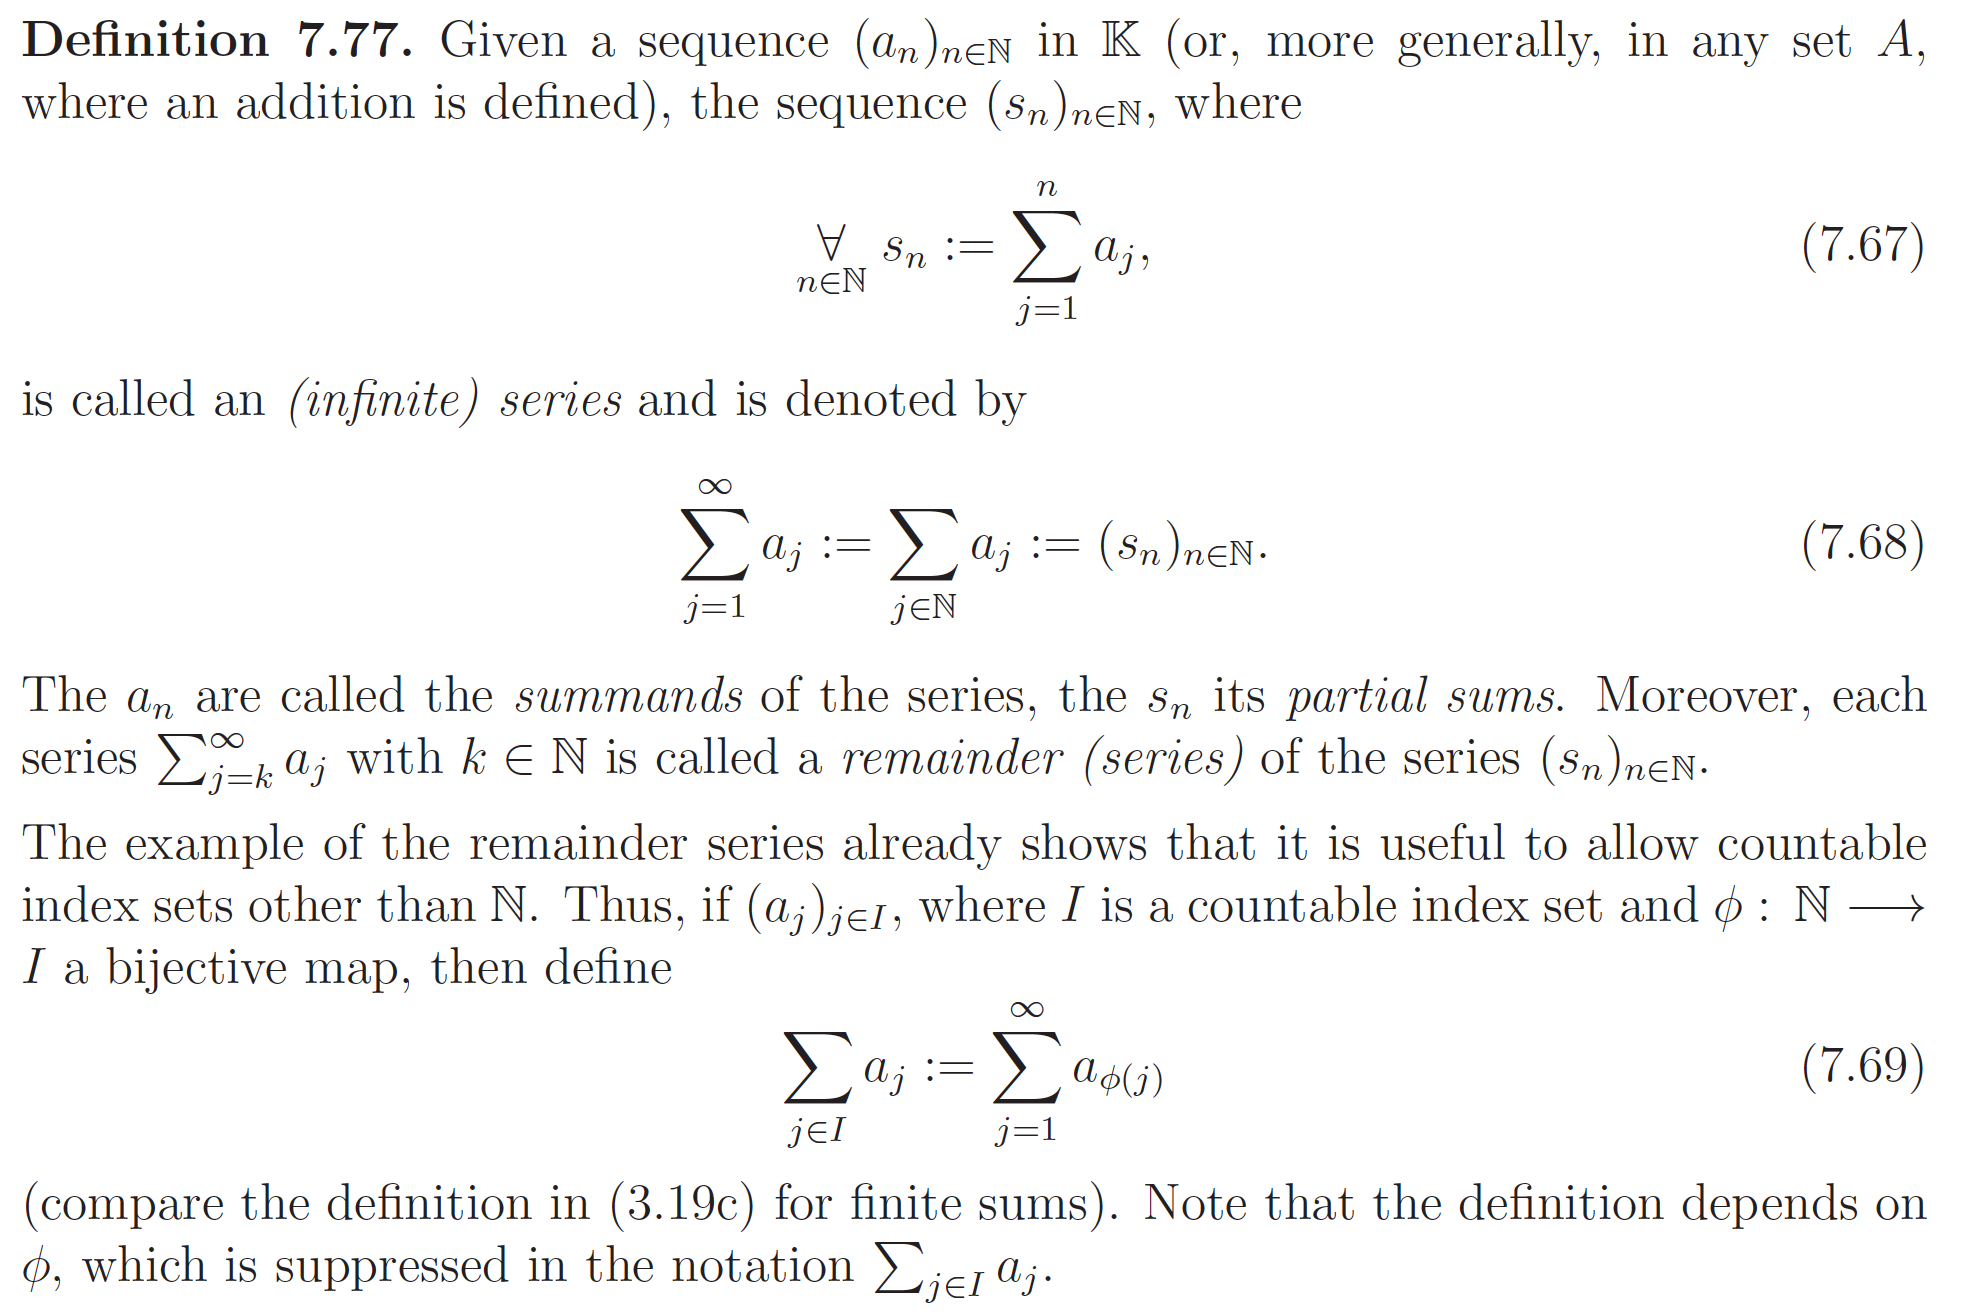
\includegraphics[width=0.7\textwidth]{media/8-1.png}
\end{figure}

\subsection{Definition von Konvergenz und Divergenz von Reihen. (96)}

\begin{figure}[H] \centering
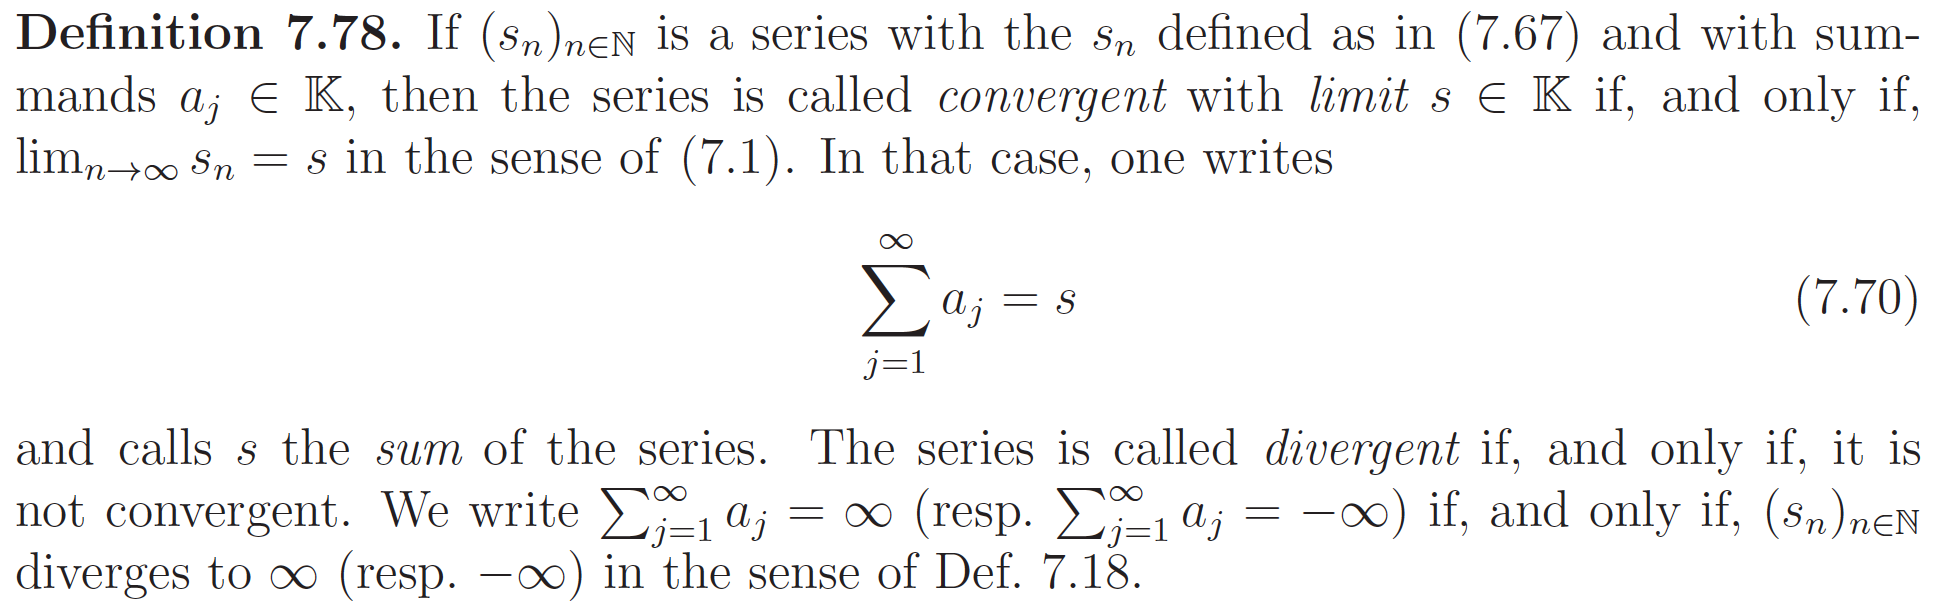
\includegraphics[width=0.7\textwidth]{media/8-2.png}
\end{figure}

\subsection{Geometrische Reihen mit Formel für den Grenzwert. (96)}

\begin{figure}[H] \centering
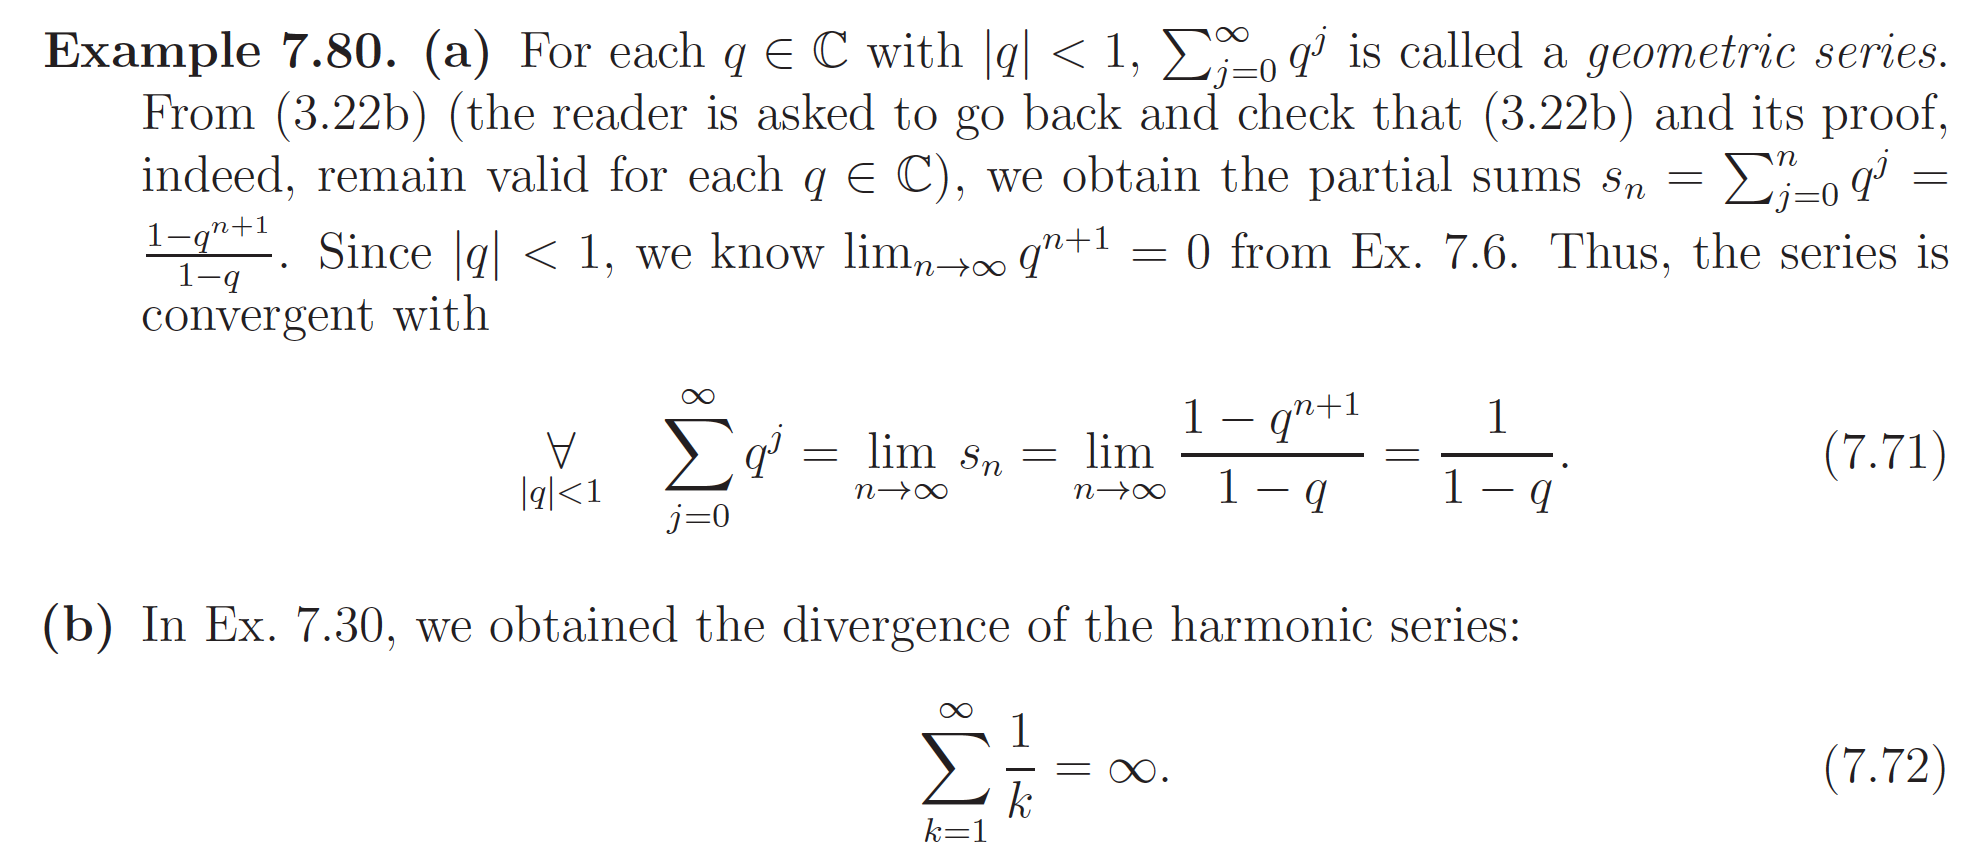
\includegraphics[width=0.7\textwidth]{media/8-3.png}
\end{figure}

\subsection{Linearität, komplexe Konjugation und Monotonie bei der Reihenkonvergenz. (96)}

\begin{figure}[H] \centering
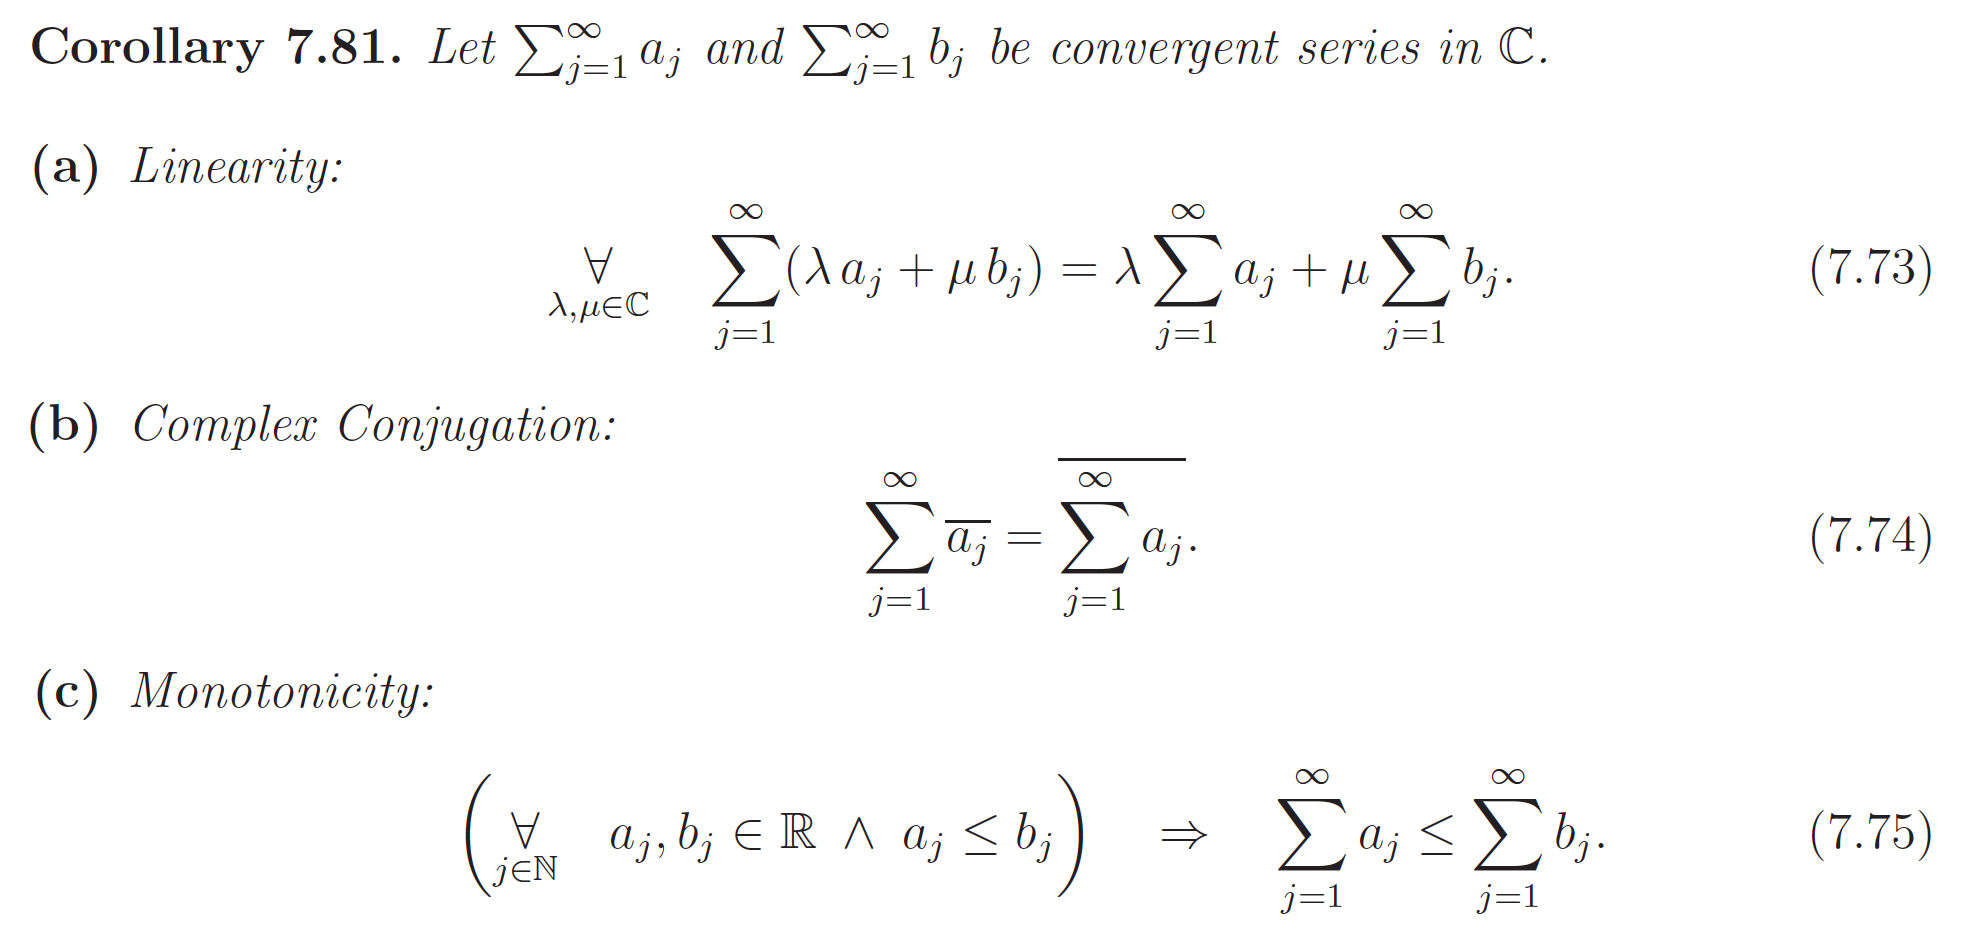
\includegraphics[width=0.7\textwidth]{media/8-4.png}
\end{figure}

\subsection{Satz: Bei konvergenten Reihen konvergieren die Summanden gegen Null. (97)}

\begin{figure}[H] \centering
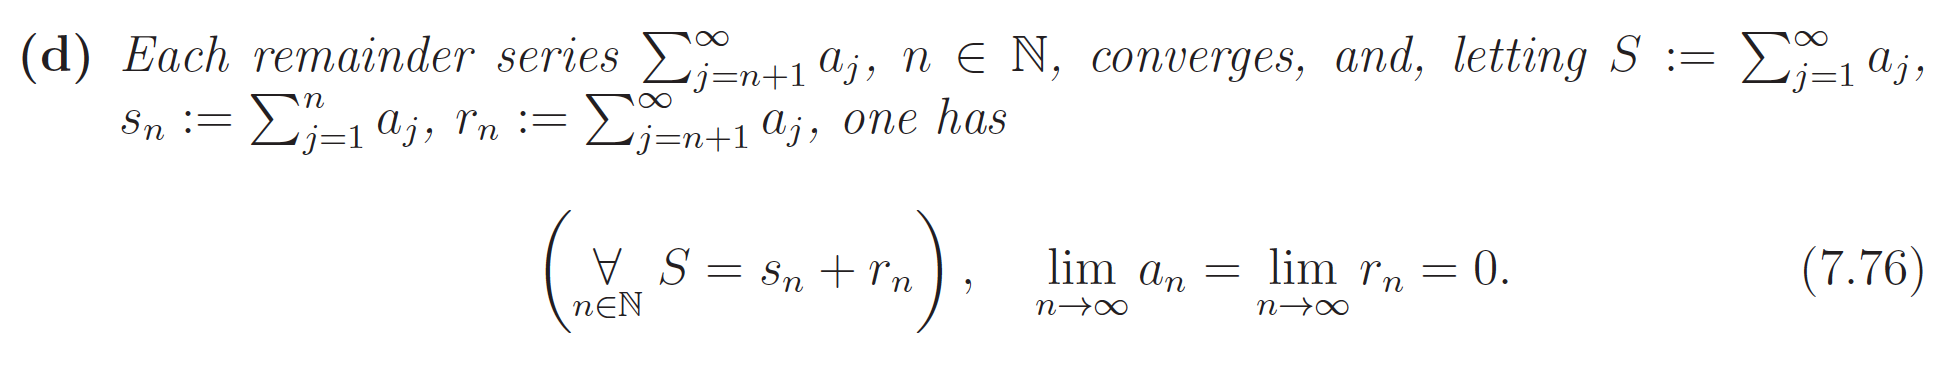
\includegraphics[width=0.7\textwidth]{media/8-5.png}
\end{figure}

\subsection{Satz: Die Summe einer Reihe mit nichtnegativen Summanden ist das Supremum der Partialsummen, wenn diese beschränkt sind und andernfalls unendlich. (97)}

\begin{figure}[H] \centering
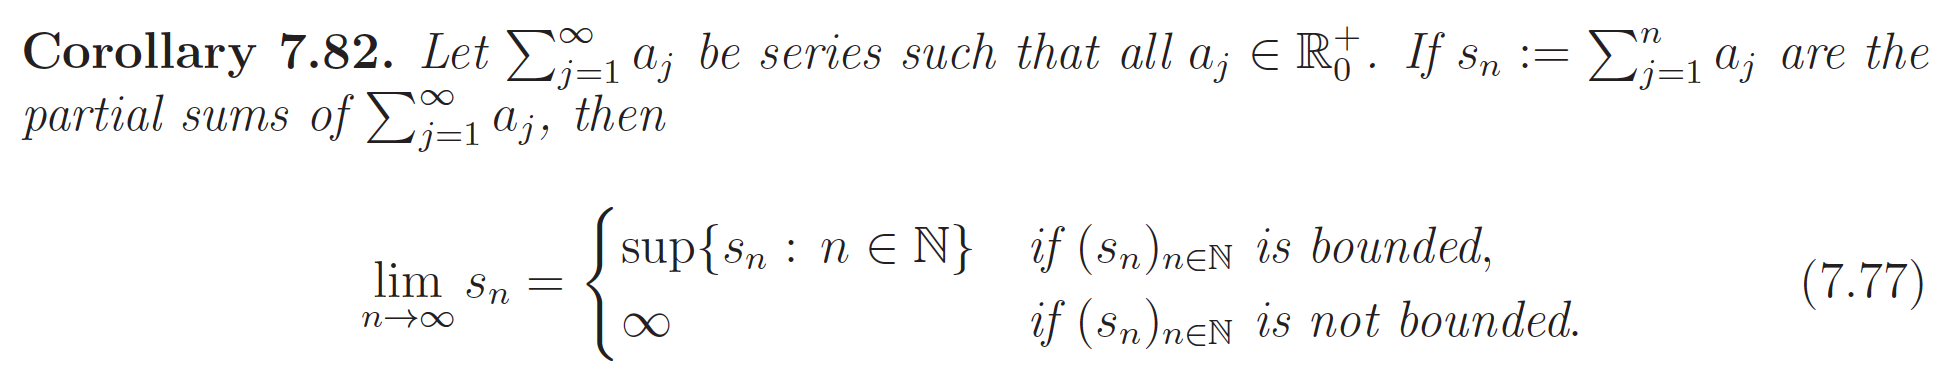
\includegraphics[width=0.7\textwidth]{media/8-6.png}
\end{figure}

\subsection{Satz: Eine beliebige Reihe ist konvergent, wenn sich die Beträge ihrer Summanden nach oben durch die Summanden einer konvergenten Reihe abschätzen lassen; eine Reihe mit nichtnegativen Summanden ist divergent, wenn sich ihre Summanden nach unten durch die Summanden einer divergenten Reihe mit ebenfalls nichtnegativen Summanden abschätzen lassen. (97)}

\begin{figure}[H] \centering
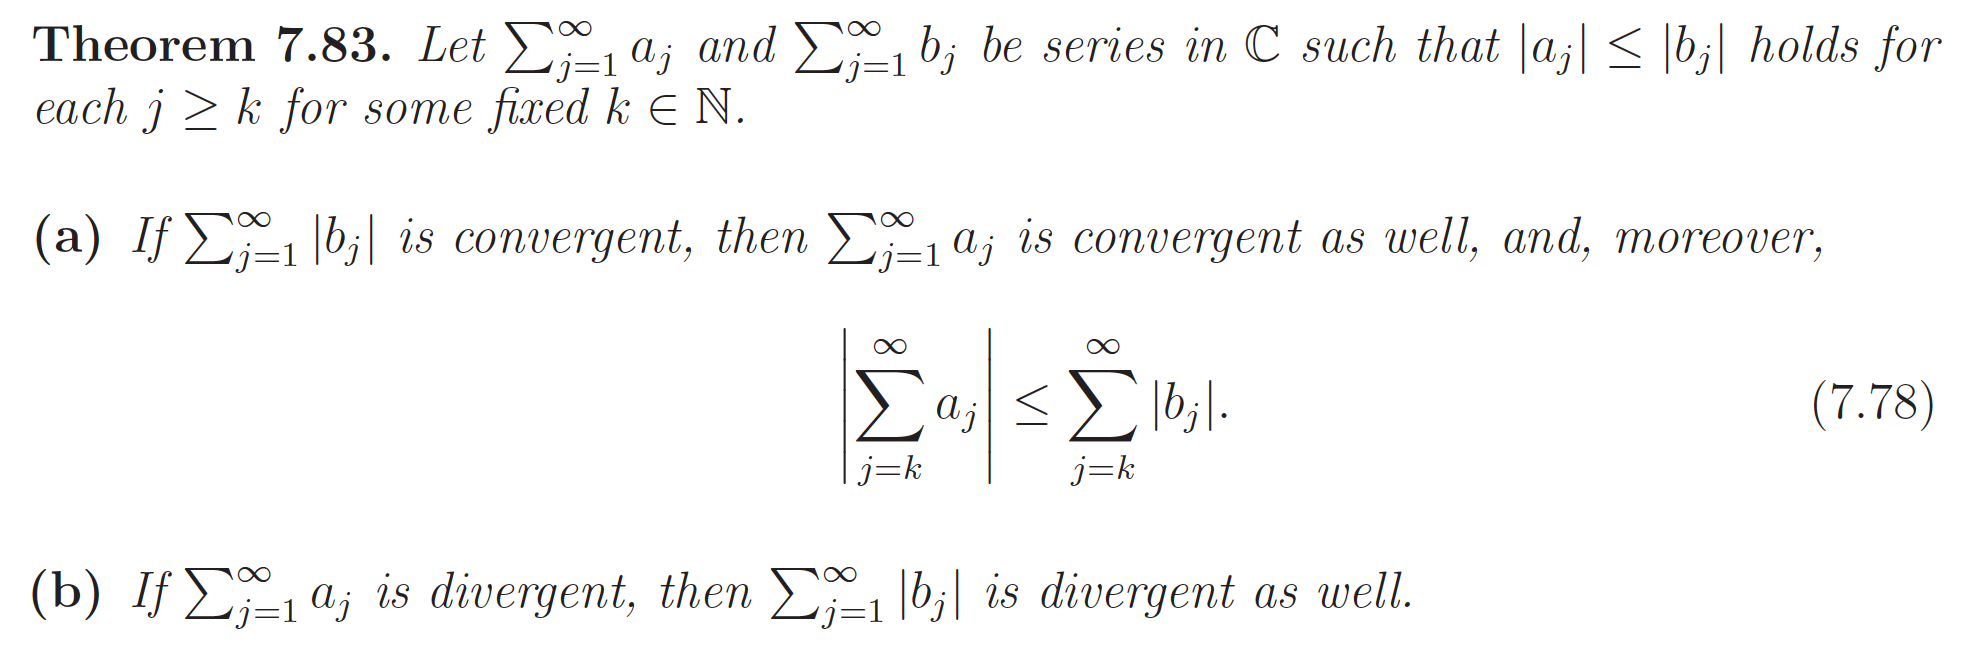
\includegraphics[width=0.7\textwidth]{media/8-7.png}
\end{figure}

\subsection{Definition der absoluten Konvergenz von Reihen. (99)}

\begin{figure}[H] \centering
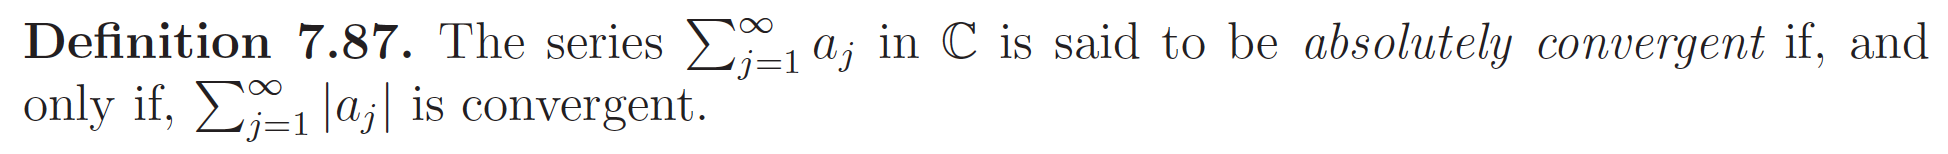
\includegraphics[width=0.7\textwidth]{media/8-8.png}
\end{figure}

\subsection{Satz: Absolut konvergente Reihen sind konvergent, und es gilt die Dreiecksungleichung für unendliche Reihen. (99)}

\begin{figure}[H] \centering
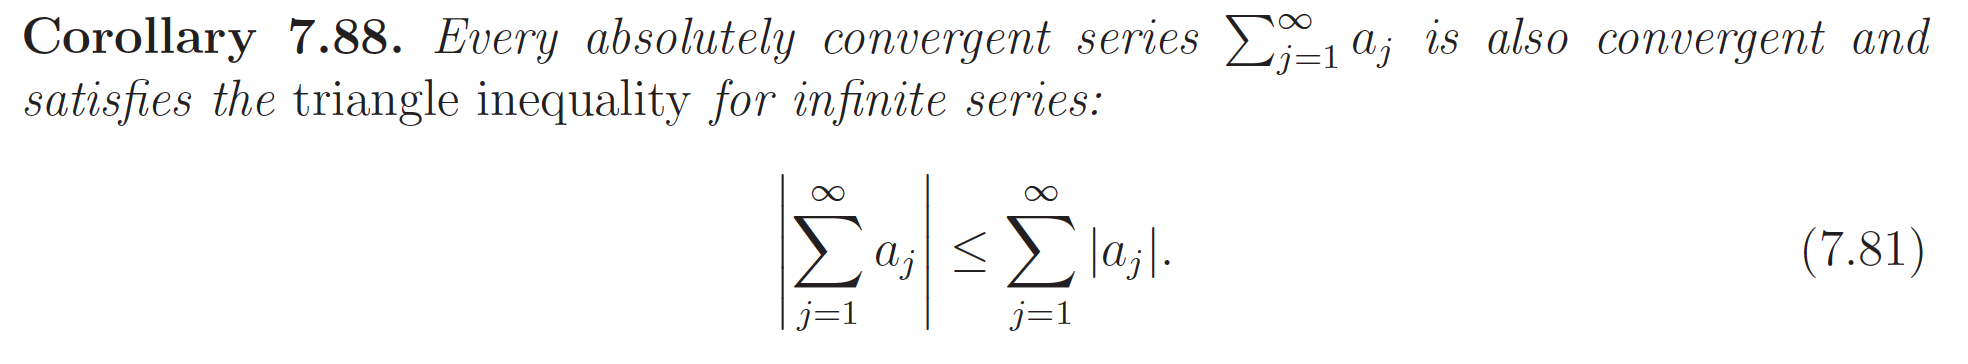
\includegraphics[width=0.7\textwidth]{media/8-9.png}
\end{figure}

\subsection{Wurzelkriterium und Quotientenkriterium jeweils für absolute Konvergenz bzw. für Divergenz. (99f)}

\begin{figure}[H] \centering
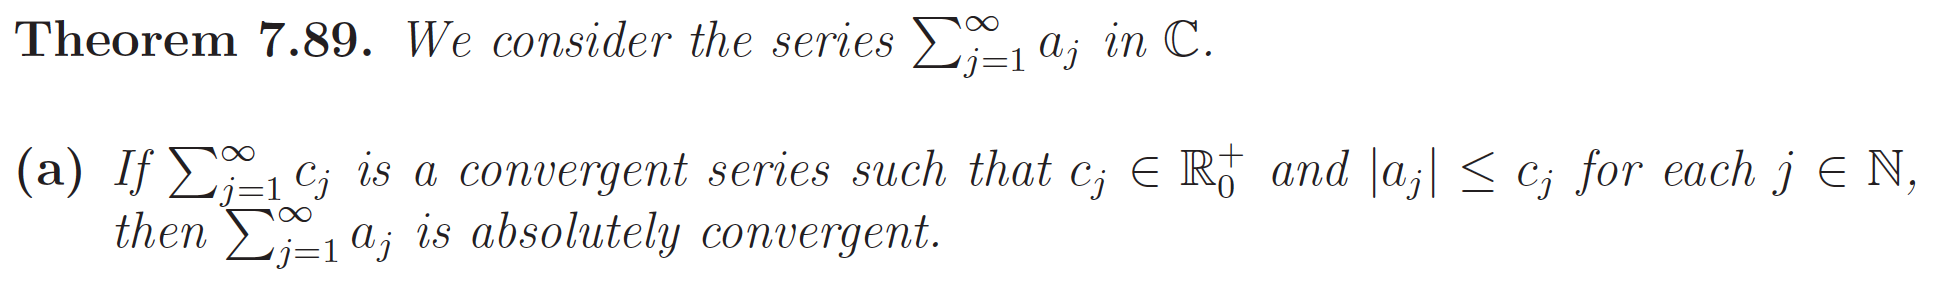
\includegraphics[width=0.7\textwidth]{media/8-10.png}
\end{figure}
\begin{figure}[H] \centering
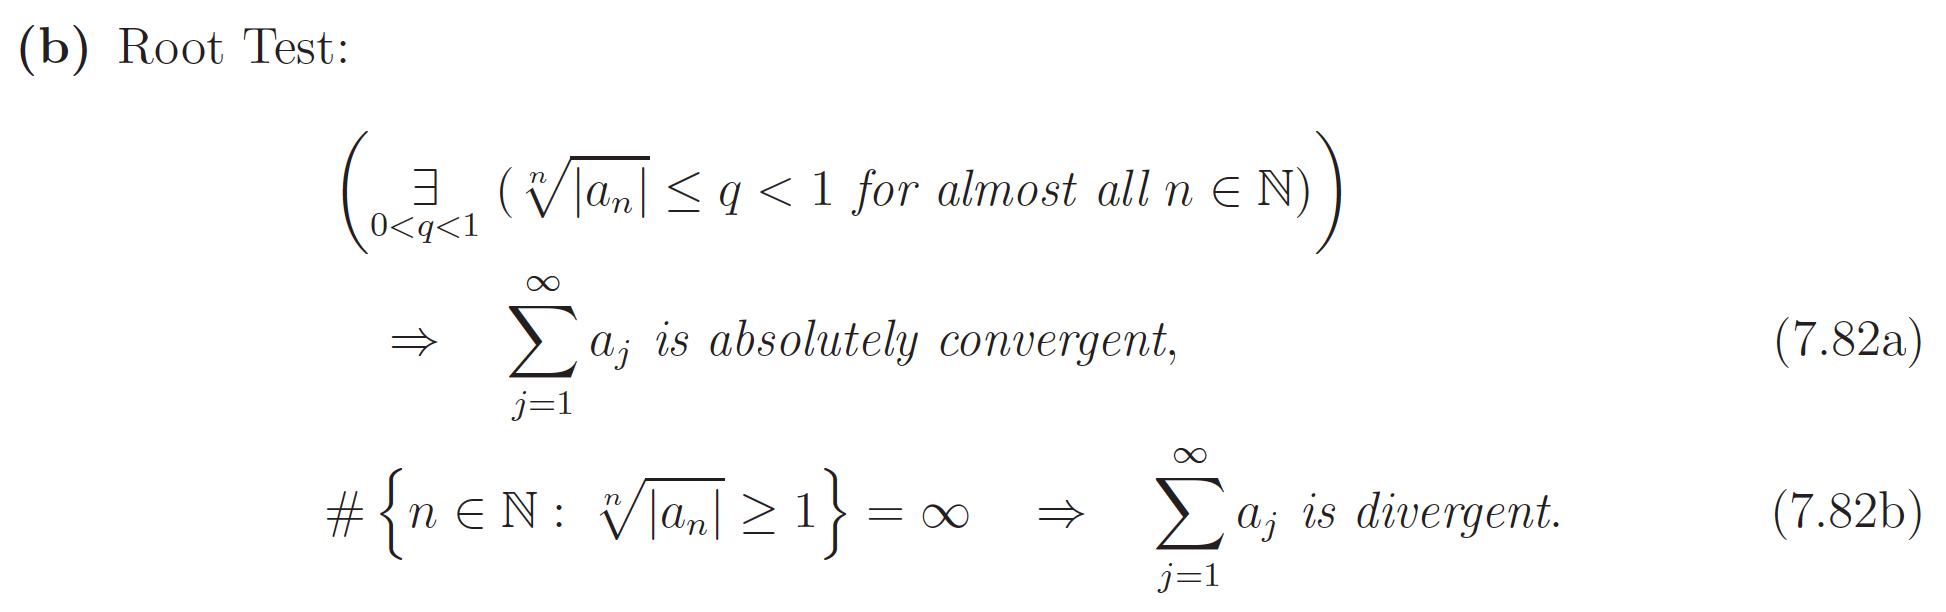
\includegraphics[width=0.7\textwidth]{media/8-10-2.png}
\end{figure}
\begin{figure}[H] \centering
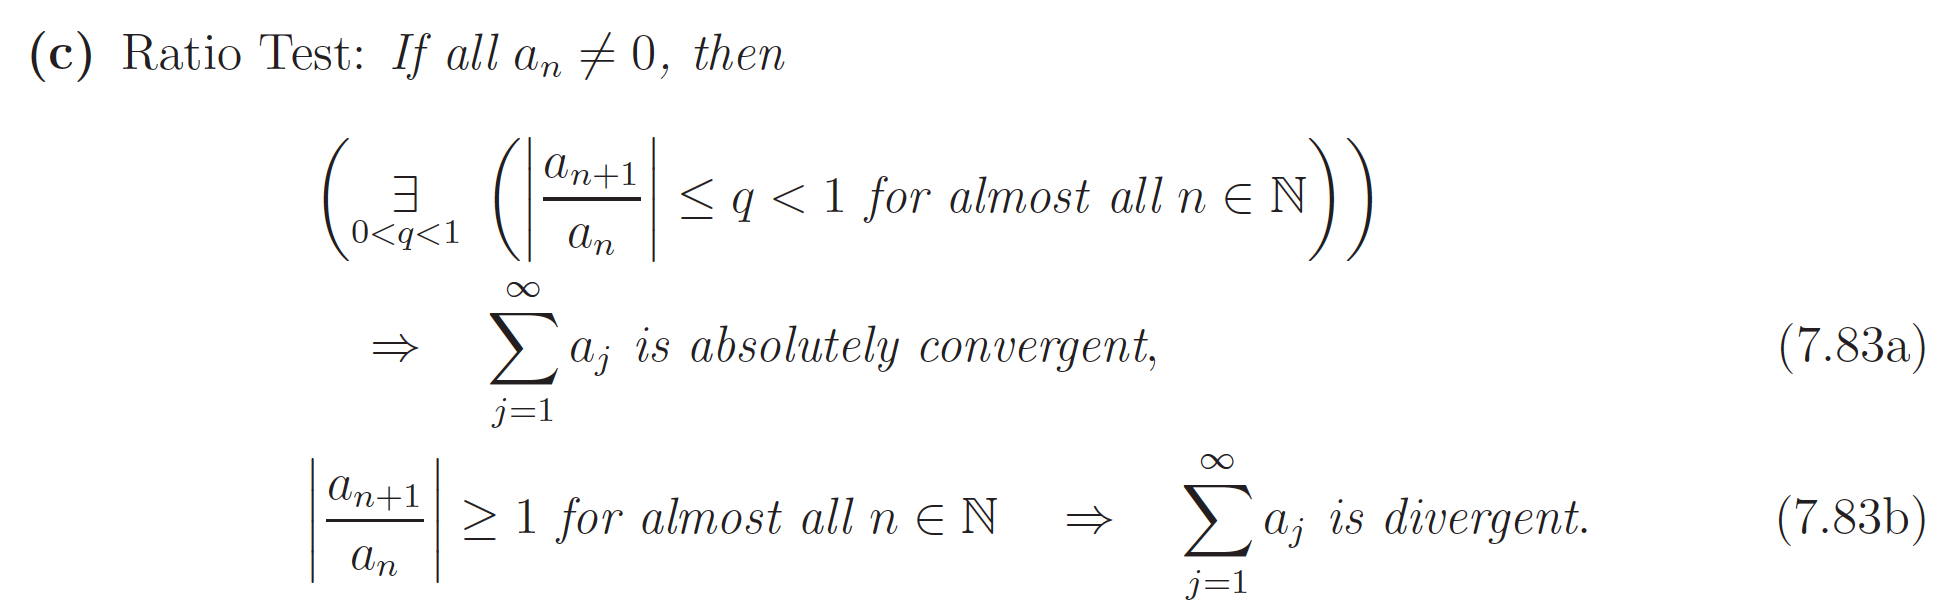
\includegraphics[width=0.7\textwidth]{media/8-10-3.png}
\end{figure}

\subsection{Definition der punktweisen und der gleichmäßigen Konvergenz von Funktionenfolgen bestehend aus reell- oder komplexwertigen Funktionen. (105)}

\begin{figure}[H] \centering
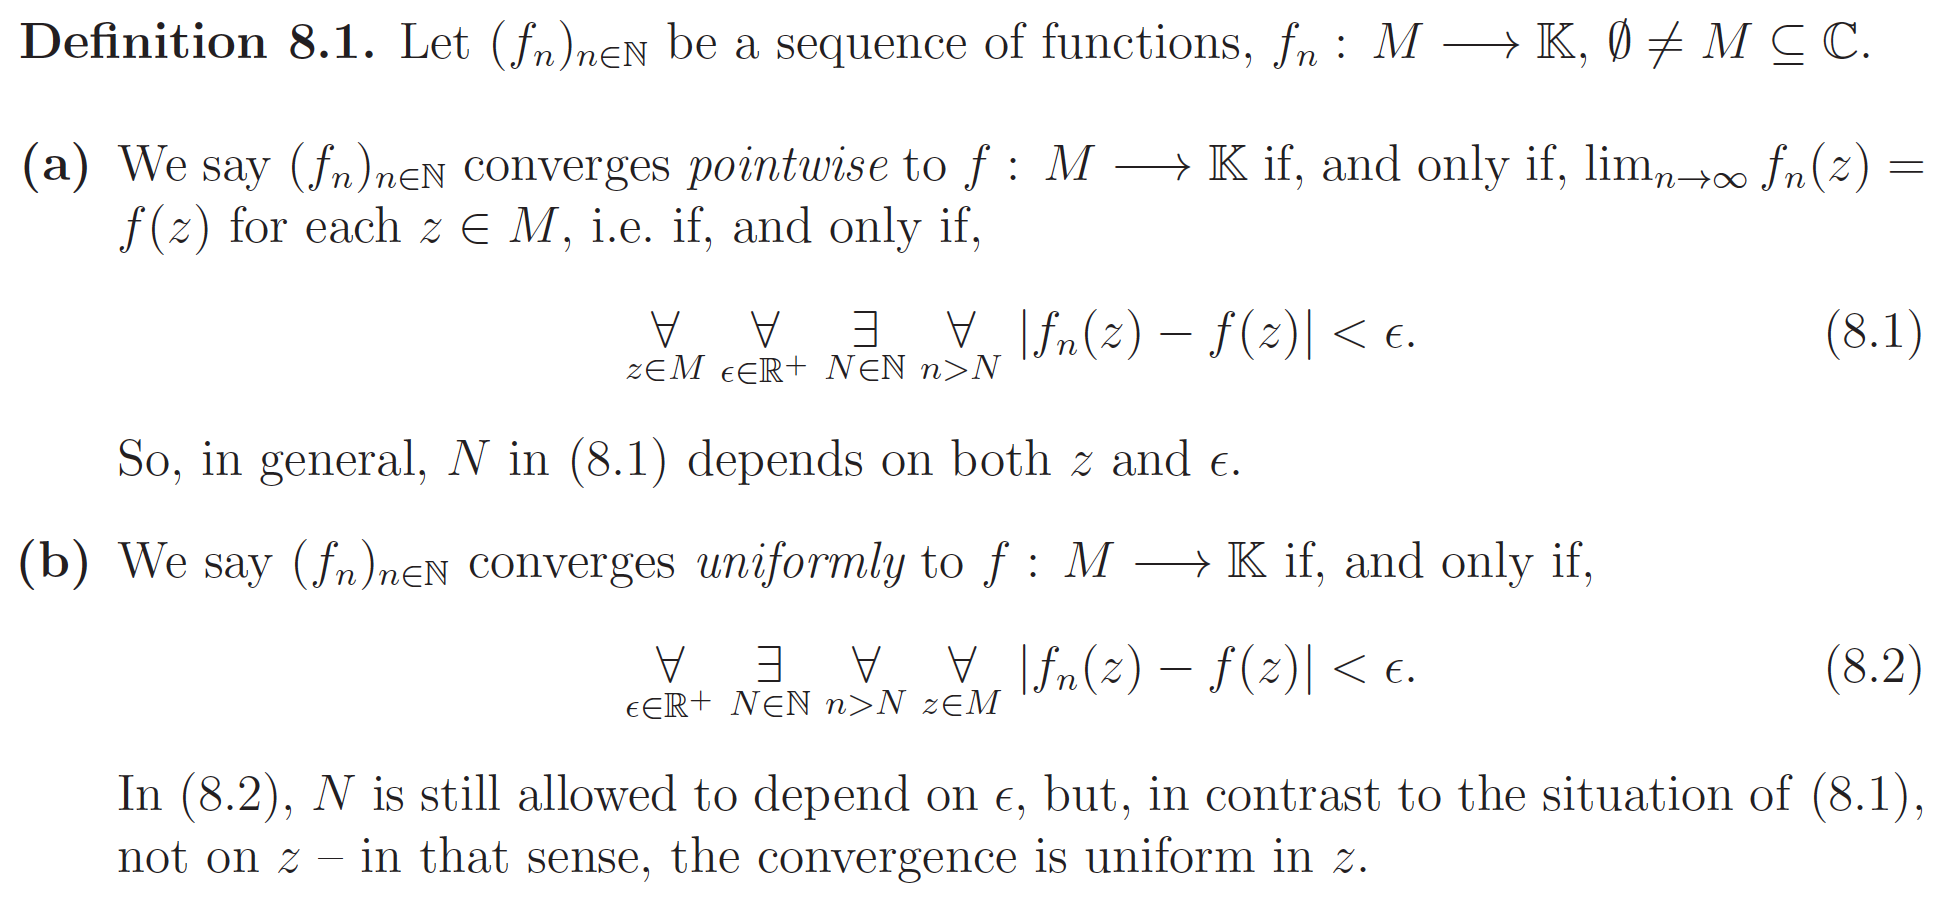
\includegraphics[width=0.7\textwidth]{media/8-11.png}
\end{figure}

\subsection{Satz: Gleichmäßige Konvergenz impliziert punktweise Konvergenz, aber nicht umgekehrt. (105)}

\begin{figure}[H] \centering
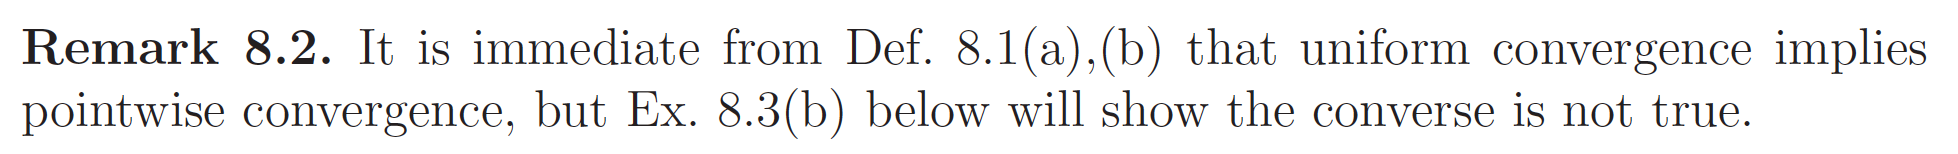
\includegraphics[width=0.7\textwidth]{media/8-12.png}
\end{figure}

\subsection{Satz: Konvergieren stetige Funktionen gleichmäßig, so ist die Grenzfunktion ebenfalls stetig. (106)}

\begin{figure}[H] \centering
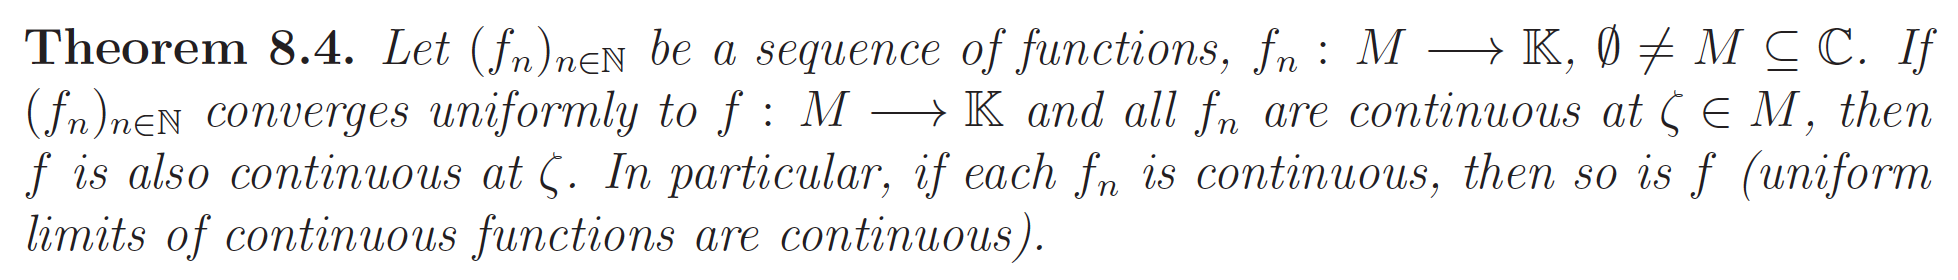
\includegraphics[width=0.7\textwidth]{media/8-13.png}
\end{figure}

\subsection{Definition von Funktionenreihen, speziell Definition von Potenzreihen. (106f)}

\begin{figure}[H] \centering
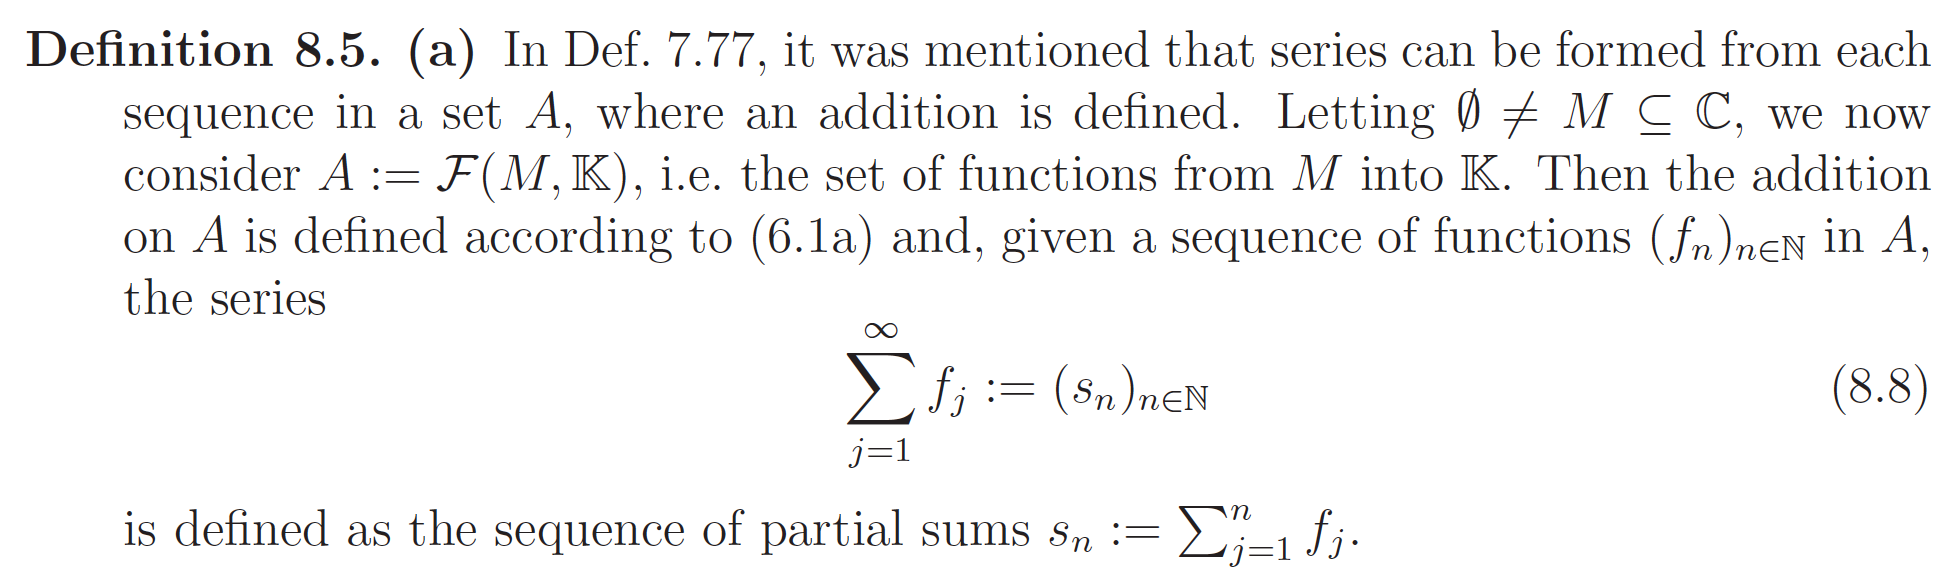
\includegraphics[width=0.7\textwidth]{media/8-14.png}
\end{figure}
\begin{figure}[H] \centering
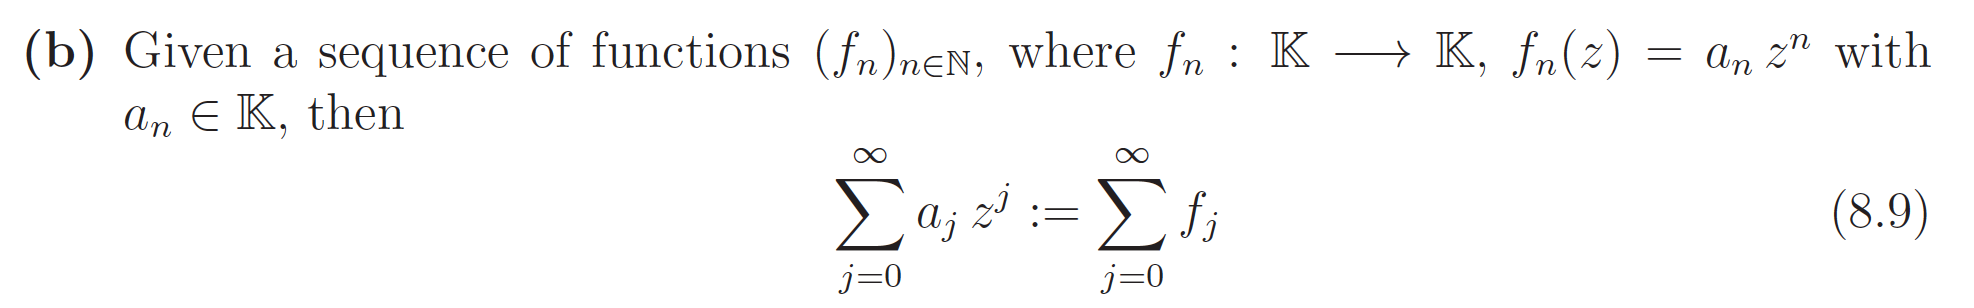
\includegraphics[width=0.7\textwidth]{media/8-14-2.png}
\end{figure}
\begin{figure}[H] \centering
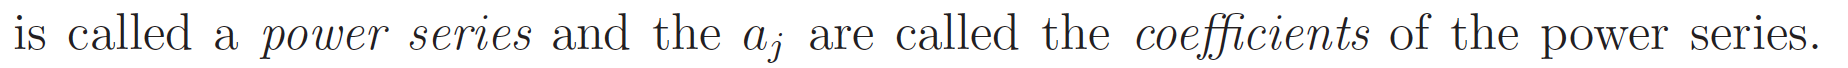
\includegraphics[width=0.7\textwidth]{media/8-14-3.png}
\end{figure}

\subsection{Definition der punktweisen und gleichmäßigen Konvergenz von Funktionenreihen (man spricht von Reihenentwicklung bzw. Potenzreihenentwicklung der Grenzfunktion). (107)}

\begin{figure}[H] \centering
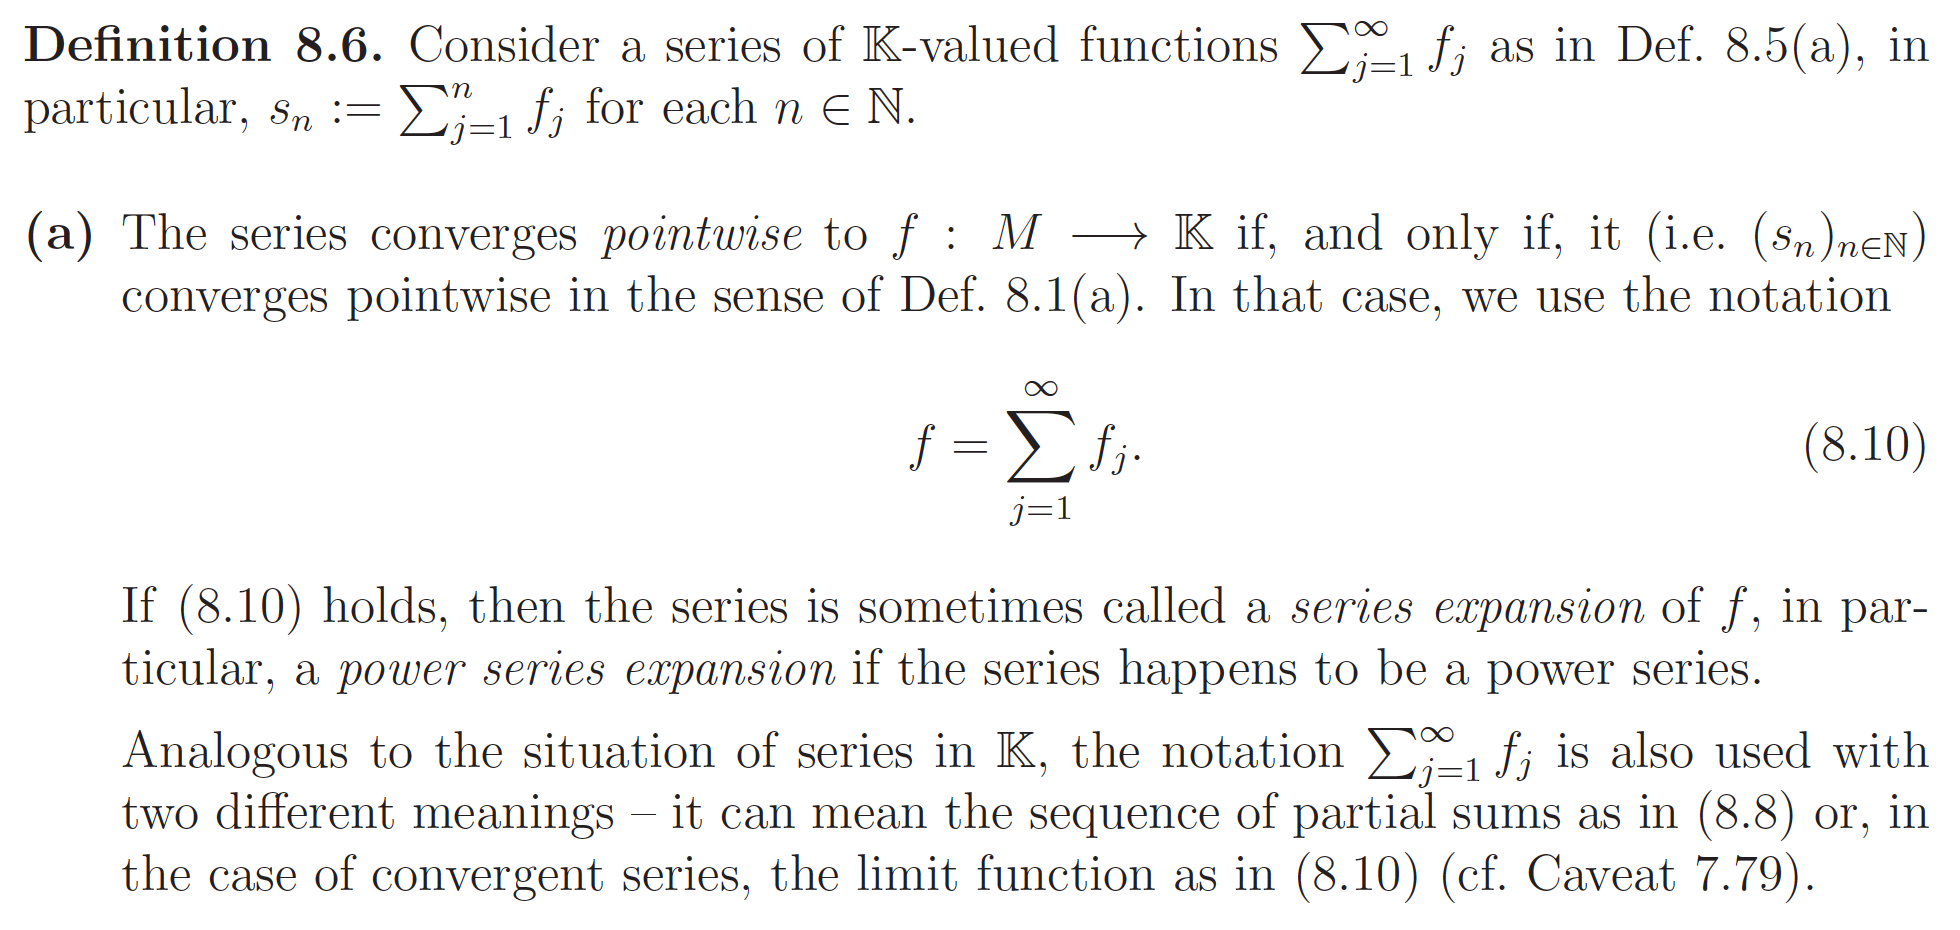
\includegraphics[width=0.7\textwidth]{media/8-15.png}
\end{figure}
\begin{figure}[H] \centering
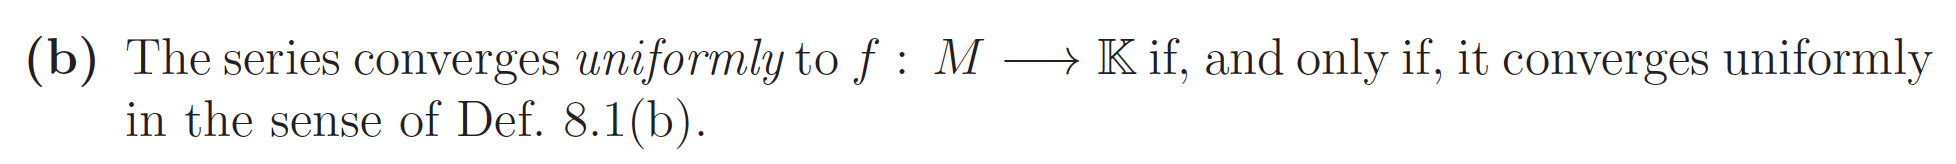
\includegraphics[width=0.7\textwidth]{media/8-15-2.png}
\end{figure}

\subsection{Konvergiert eine Funktionenreihe stetiger Funktionen gleichmäßig, so ist die Grenzfunktion stetig. (107)}

\begin{figure}[H] \centering
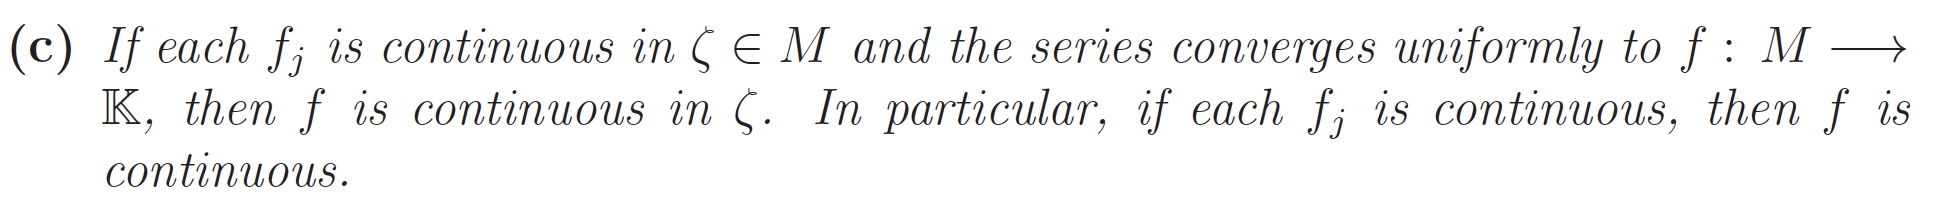
\includegraphics[width=0.7\textwidth]{media/8-16.png}
\end{figure}

\subsection{Definition des Konvergenzradius und Formeln zur Berechnung des Konvergenzradius von Potenzreihen. (108)}

\begin{figure}[H] \centering
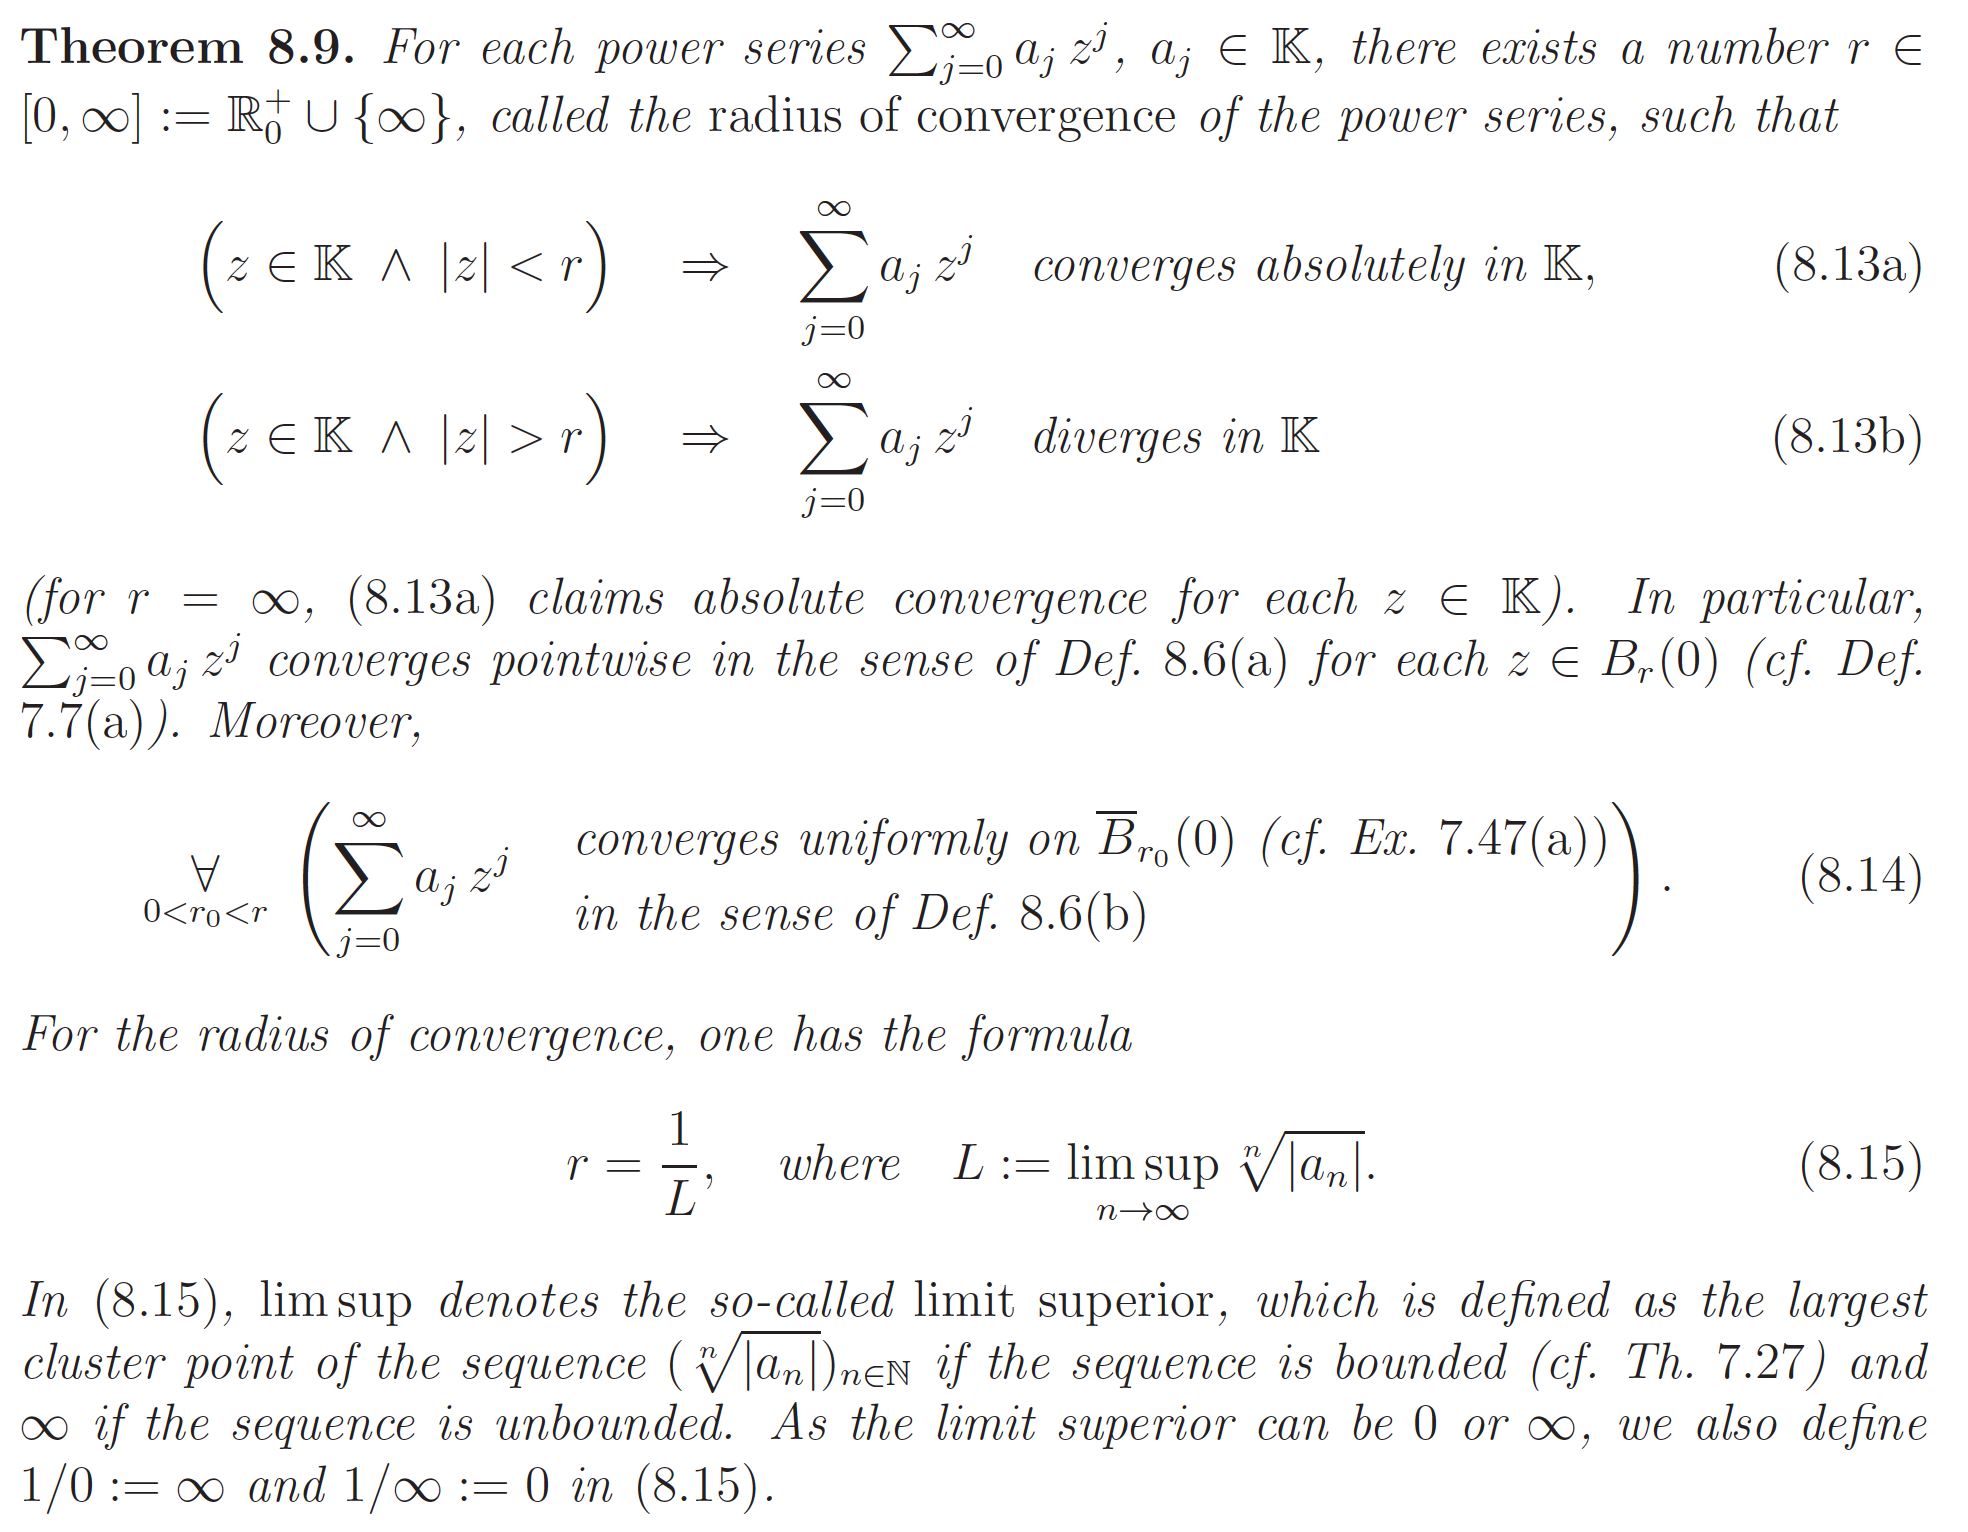
\includegraphics[width=0.7\textwidth]{media/8-17.png}
\end{figure}
\begin{figure}[H] \centering
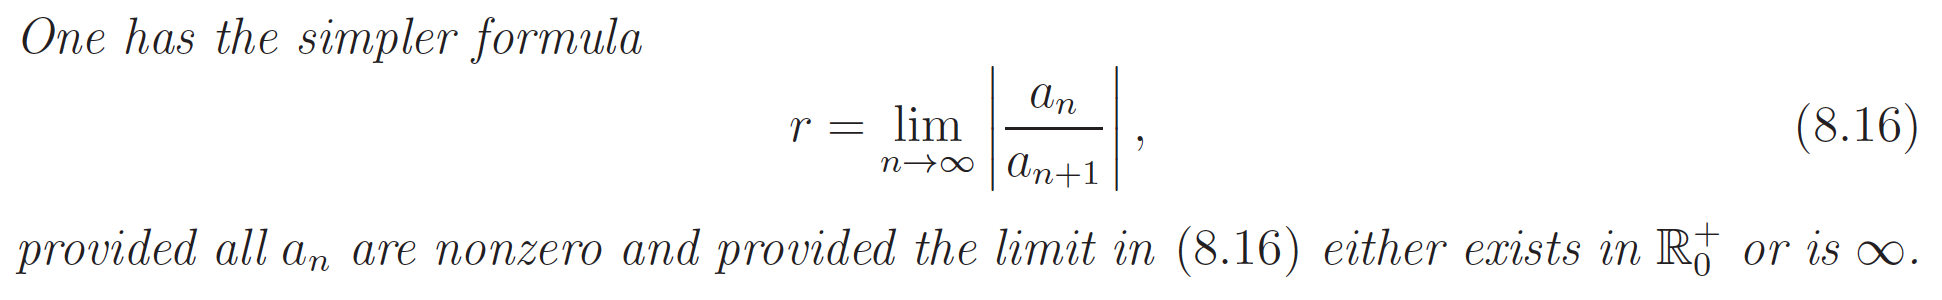
\includegraphics[width=0.7\textwidth]{media/8-17-2.png}
\end{figure}

\subsection{Satz: Potenzreihen sind auf auf dem offenen r-Kreis um Null stetig, wenn r der Konvergenzradius ist. (109)}

\begin{figure}[H] \centering
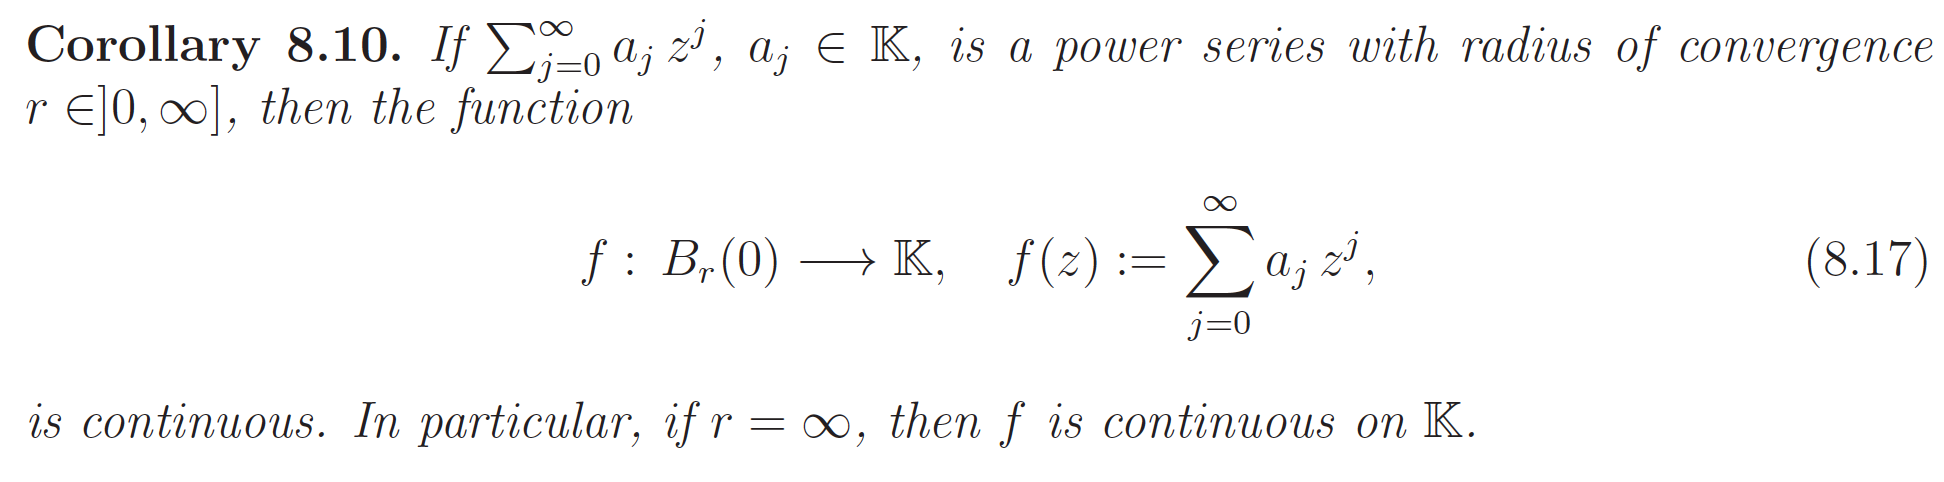
\includegraphics[width=0.7\textwidth]{media/8-18.png}
\end{figure}

\subsection{Definition der komplexen Exponentialfunktion als Potenzreihe. (111)}

\begin{figure}[H] \centering
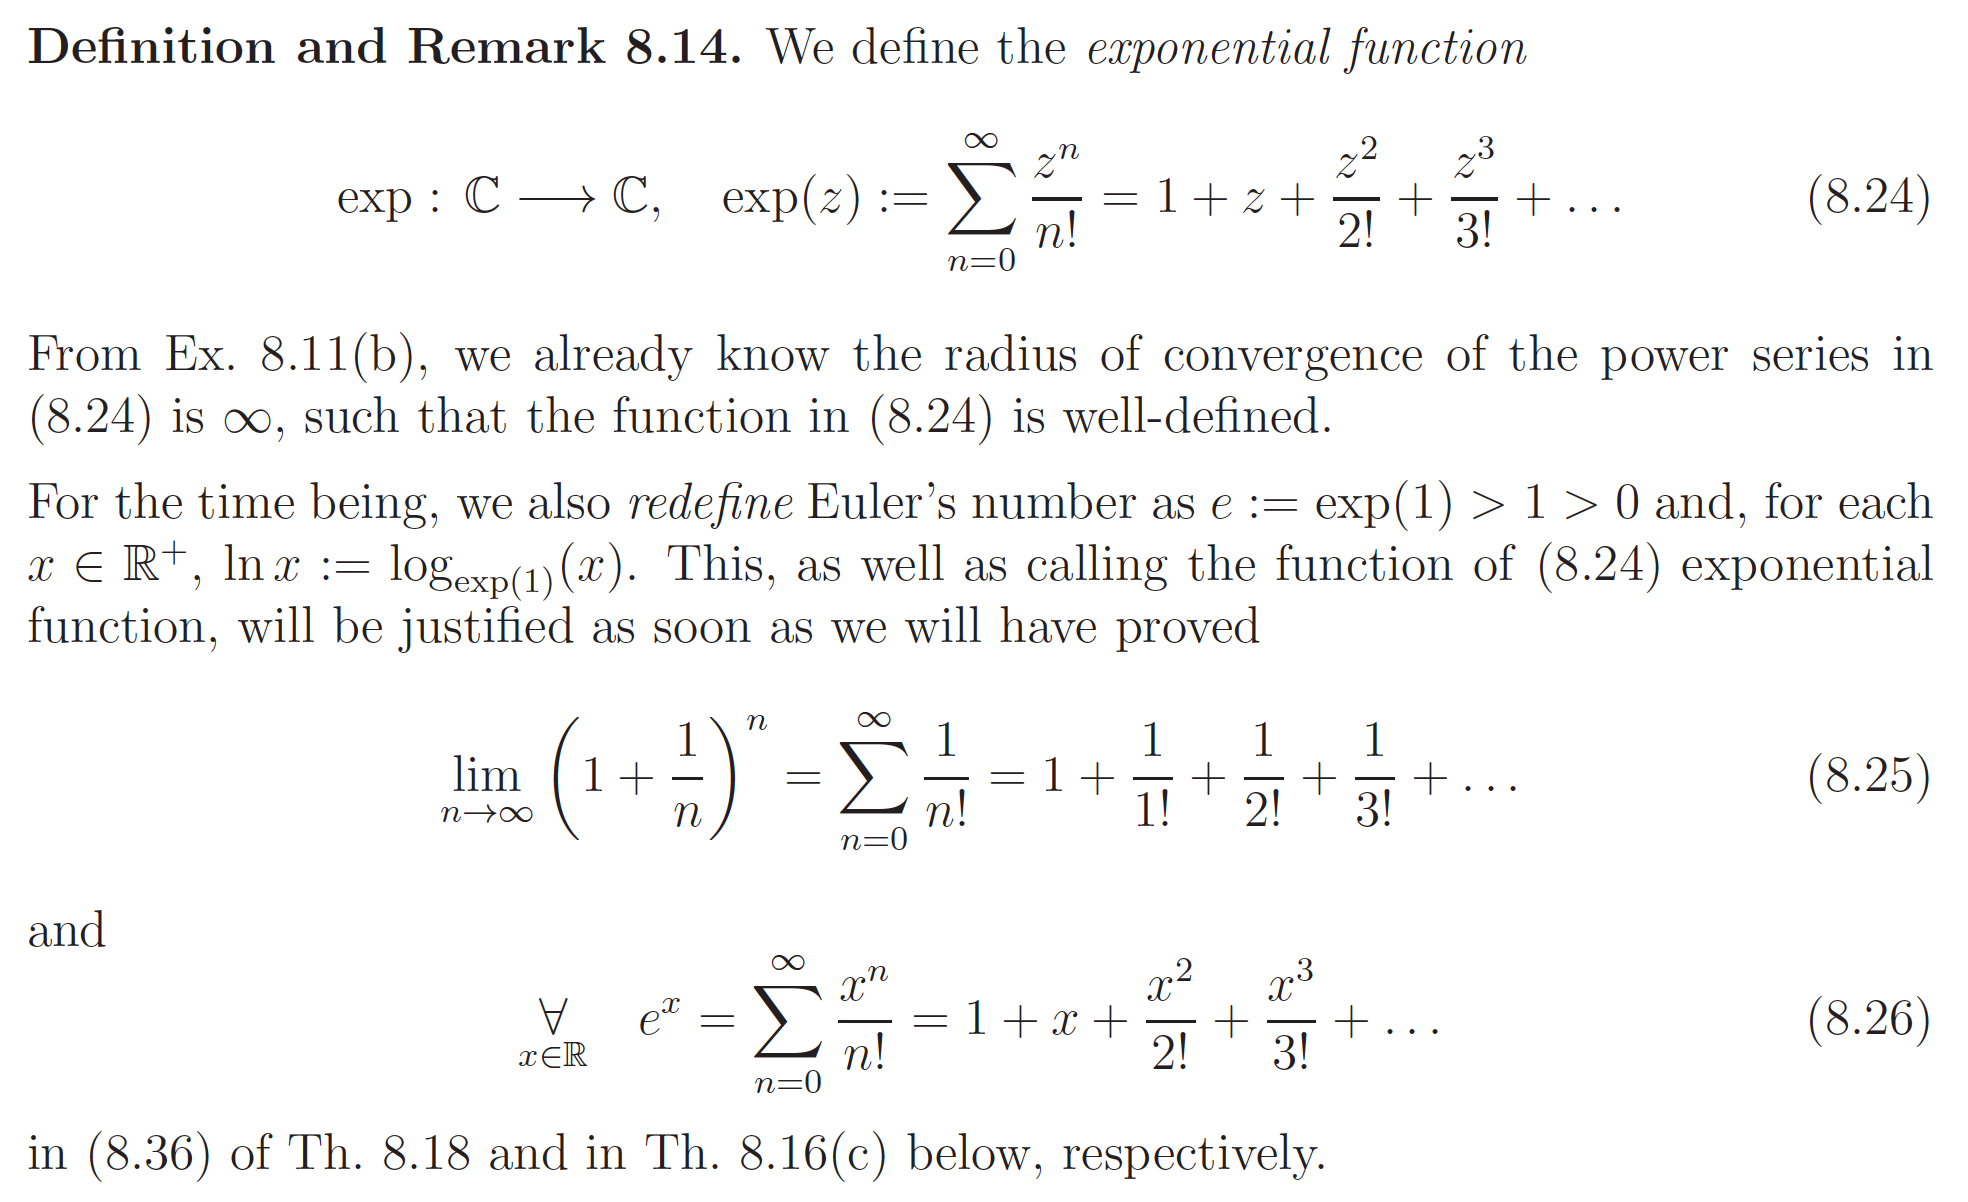
\includegraphics[width=0.7\textwidth]{media/8-19.png}
\end{figure}

\subsection{Satz: Die komplexe Exponentialfunktion ist stetig und stimmt auf den reellen Zahlen mit der früher definierten Exponentialfunktion überein. (111)} 

\begin{figure}[H] \centering
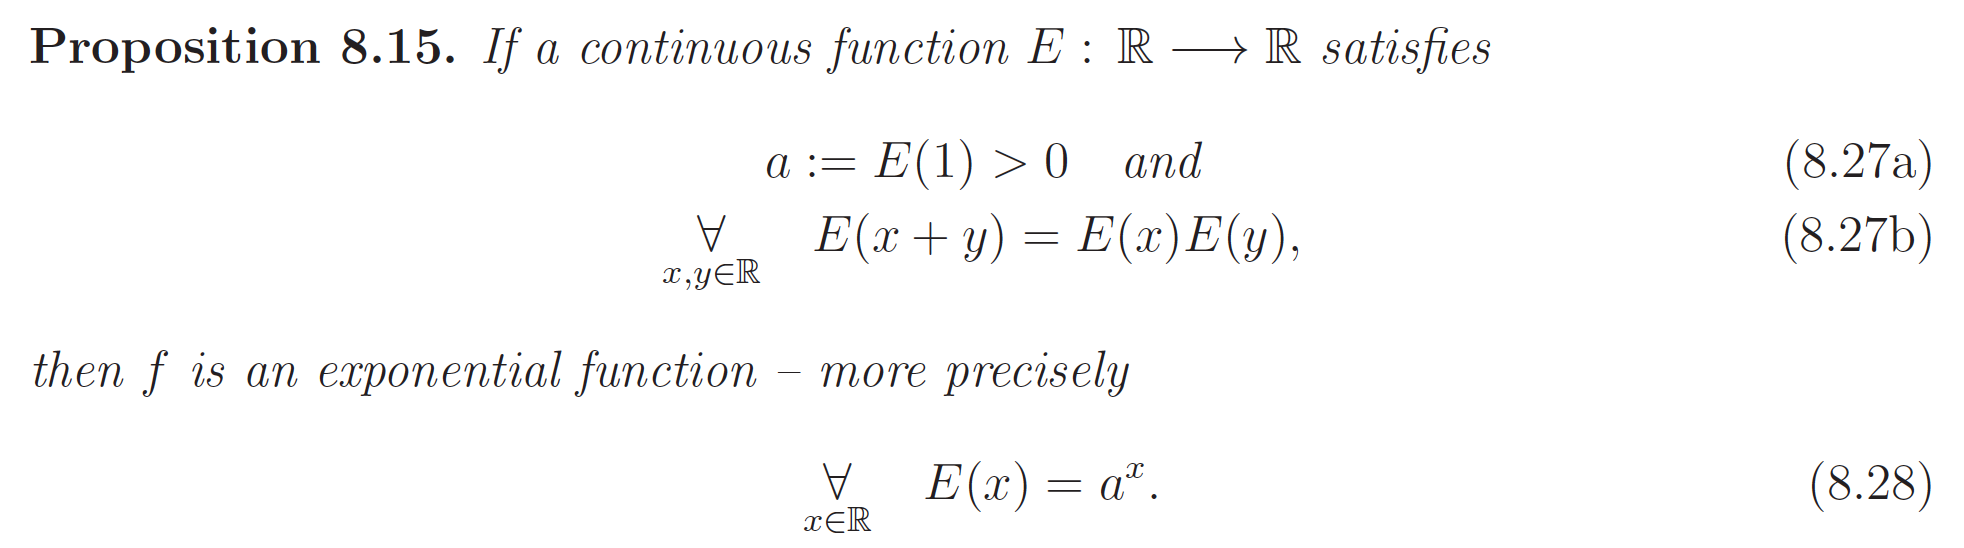
\includegraphics[width=0.7\textwidth]{media/8-20.png}
\end{figure}

\subsection{Definition des Limes einer reell- oder komplexwertigen Funktion. (112)}

\begin{figure}[H] \centering
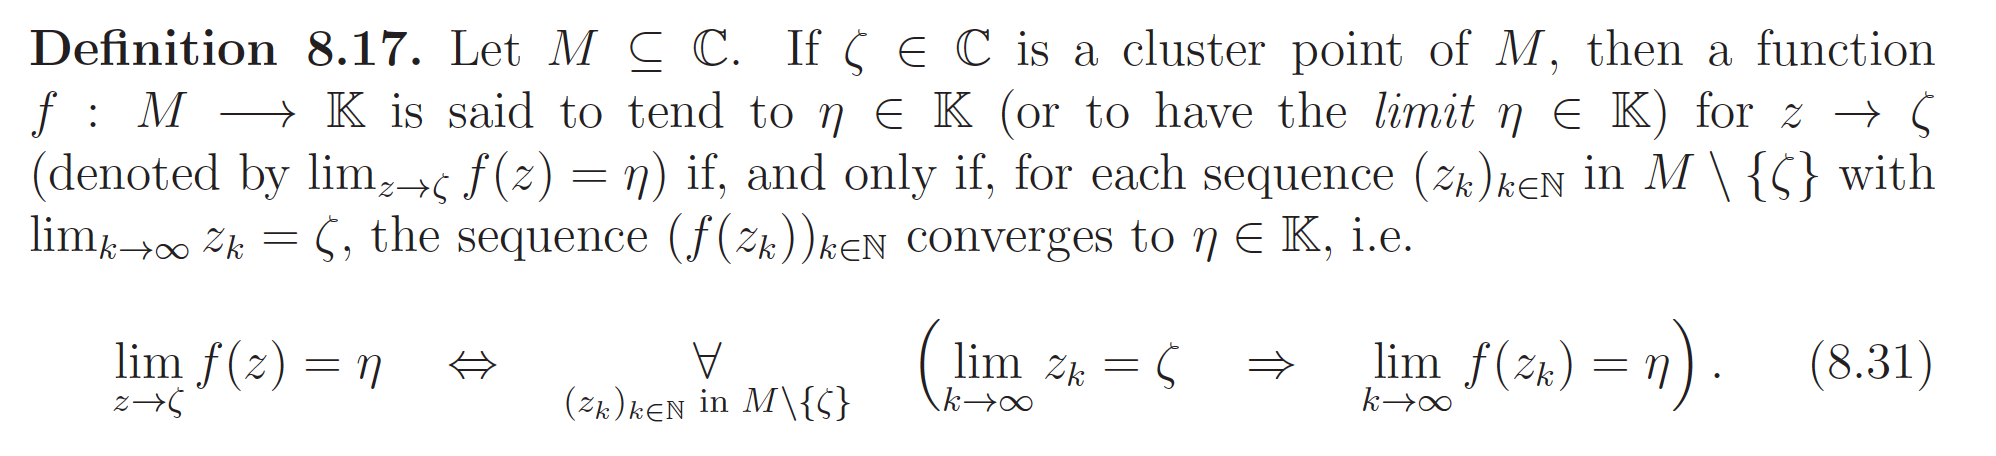
\includegraphics[width=0.7\textwidth]{media/8-21.png}
\end{figure}

\subsection{Definition von Potenzen mit positiver Basis und komplexen Exponenten, dazu Potenzgesetze und Stetigkeit der nun allgemeineren Potenz- und Exponentialfunktionen. (113f)}

\begin{figure}[H] \centering
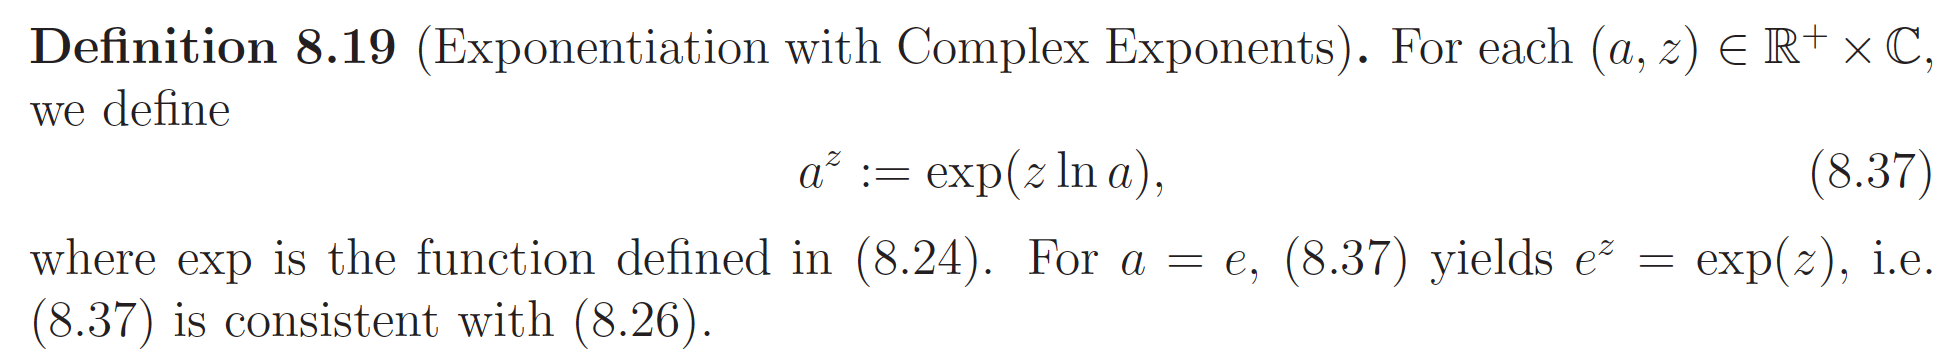
\includegraphics[width=0.7\textwidth]{media/8-22.png}
\end{figure}
\begin{figure}[H] \centering
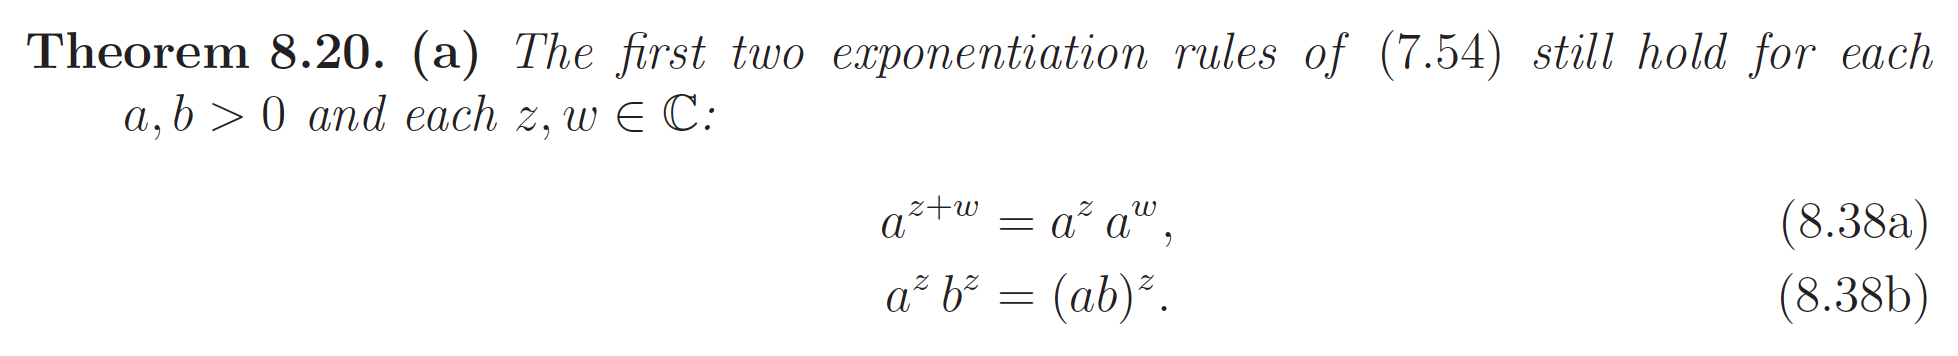
\includegraphics[width=0.7\textwidth]{media/8-22-2.png}
\end{figure}
\begin{figure}[H] \centering
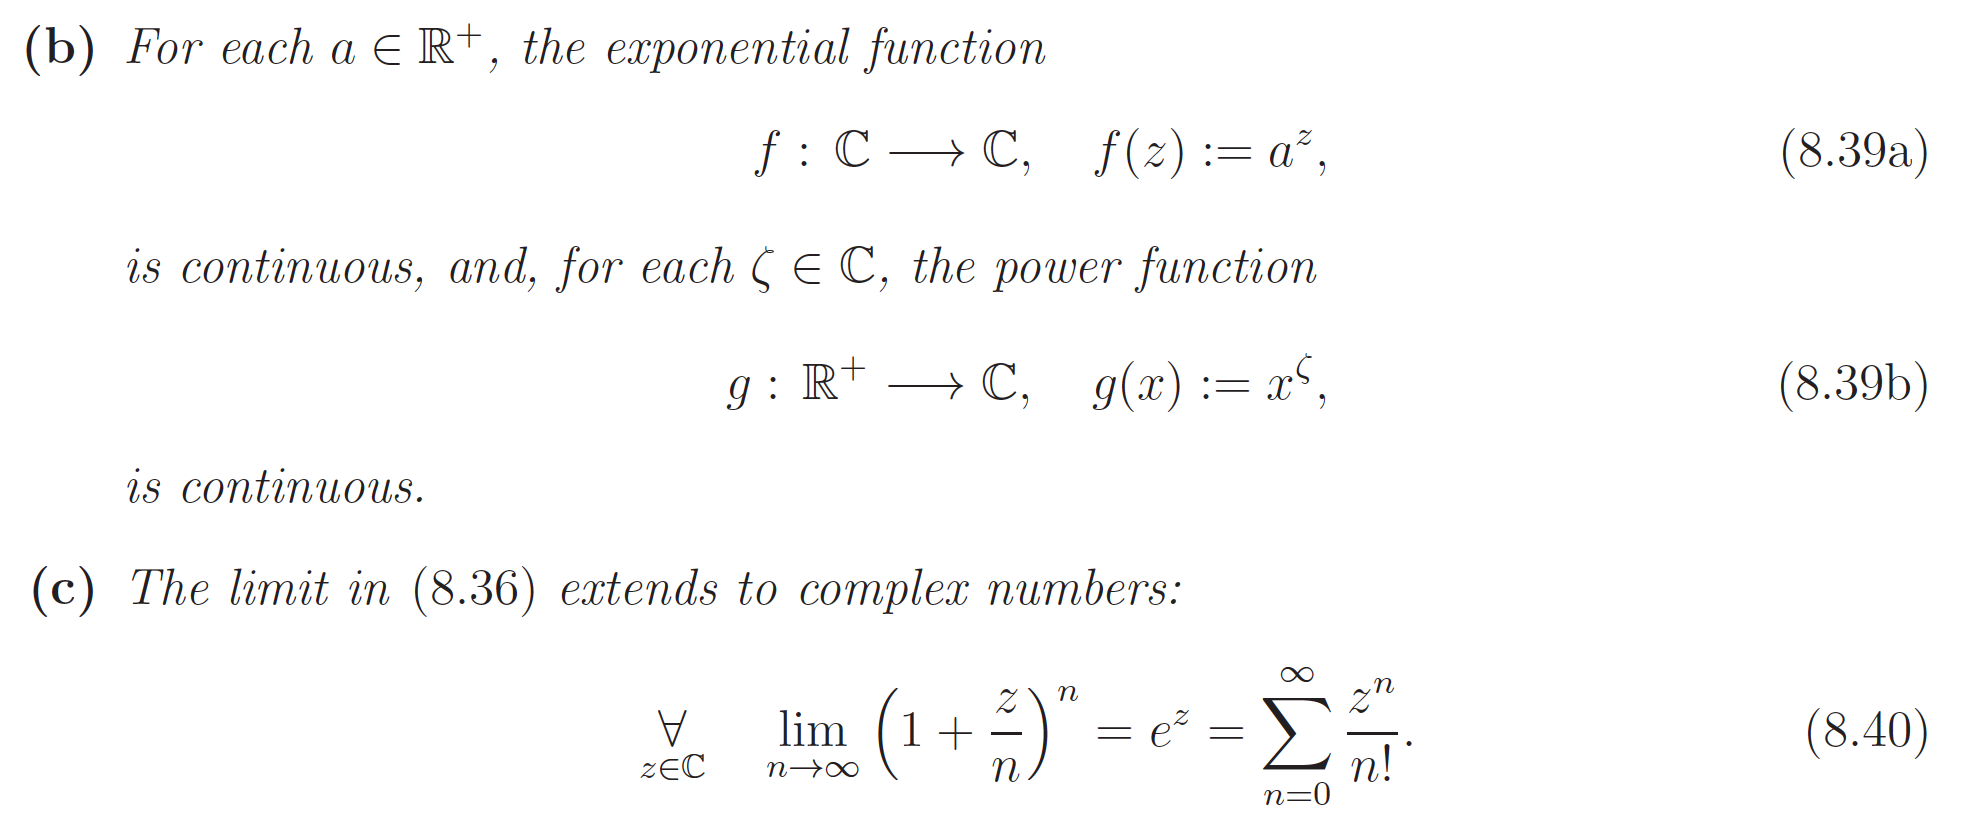
\includegraphics[width=0.7\textwidth]{media/8-22-3.png}
\end{figure}